\documentclass[11pt]{article}
\usepackage{amsmath,amssymb,amsthm}
\usepackage[margin=1in]{geometry}
\usepackage{booktabs}
\usepackage{array}
\usepackage{graphicx}
\usepackage{caption}
\usepackage{tikz}
\usetikzlibrary{arrows.meta,positioning,calc,decorations.pathreplacing}
\usepackage[hidelinks]{hyperref}

\newtheorem{theorem}{Theorem}[section]
\newtheorem{lemma}[theorem]{Lemma}
\newtheorem{proposition}[theorem]{Proposition}
\newtheorem{corollary}[theorem]{Corollary}
\newtheorem{conjecture}[theorem]{Conjecture}
\newtheorem*{theorem*}{Main Theorem}
\theoremstyle{definition}
\newtheorem{definition}[theorem]{Definition}
\newtheorem{example}[theorem]{Example}
\theoremstyle{remark}
\newtheorem{remark}[theorem]{Remark}

\newcommand{\C}{\operatorname{C}}
\newcommand{\B}{\operatorname{B}}
\definecolor{rail1}{HTML}{2A78D6}
\definecolor{rail2}{HTML}{EB6834}
\definecolor{ink2}{HTML}{52514E}

\title{Carries, Rails and Resonance:\\ the Structure of the Digit-Sum Parity Map}
\author{Rudraneel Das\\ \small Independent Researcher \quad \texttt{rudraneel93@gmail.com}\\ \small ORCID: 0009-0009-6173-0262}
\date{}

\begin{document}
\maketitle

\begin{abstract}
Let $s(n)$ be the sum of the decimal digits of $n$ and let $f(n)=n+s(n)$ for
odd $n$ and $f(n)=n-s(n)$ for even $n$. Our main result concerns the
$2$-cycles of $f$, which are most of its observed cycles. We prove that an odd
$a$ lies on a $2$-cycle if and only if $s(a)$ is odd and the addition
$a+s(a)$ produces exactly $s(s(a))/9$ carries, and we show that this
required number is within $1/9$ of the \emph{mean} number of carries produced
by adding $s(a)$ to a random odd integer (a ``carry balance'' identity).
Combining this with exchangeability of digits, an anti-concentration lemma
for carries and a local limit argument, we prove that the number of
$2$-cycles below $N$ is of exact order $N/\sqrt{\log\log N}$. In particular
$2$-cycles have density zero, so their number does not grow linearly in
$N$, although numerically they make up most of the observed cycles. We also obtain an asymptotic formula for the $2$-cycle density with
error $O((\log D)^2/\sqrt D)$ below $10^D$. Combining it with an exact formula
for the variance of the carry count and a sharp local limit theorem, we prove
an oscillation law: $\sqrt{\log_{10}D}\,T(D)/10^D$ has no limit, its limit
points form the interval $[K_0\sqrt{726/301},\,K_0\sqrt6]$ with
$K_0=1/(12\sqrt{11\pi})$, and the peak-to-trough ratio is
$\sqrt{301}/11\approx1.577$.

Along the way we establish several exact structural facts: on multiples of
nine, $f$ is conjugate to $m\mapsto m\pm\kappa(m)$ with $\kappa(m)=s(9m)/9$
given by a digit formula; a general level equation describes how the digit
sum changes under each step; a \emph{conditional} time-reversal identity
$f(f(x)+9)=x+9$ holds whenever $s(x)$ is even and $s(f(x)+9)=s(x)$; and the
orbit of $H\cdot10^L+x$ depends on $H$ only through $s(H)$ while it stays in
one prefix block, which yields a cycle-counting algorithm with a rigorous
error bound. We prove that an orbit is eventually periodic if and only if its
digit sums are bounded, and that every run of the orbit along which the
digit sum stays constant moves it by at most $O(k^2)$, where $9k$ is that digit
sum. Using this and prefix lifting we give a computer-assisted proof that
every orbit starting below $10^{2224}$ is eventually periodic (and, for the
binary analogue, every orbit starting below $2^{3024}$). Whether \emph{every}
orbit is eventually periodic remains open. It would follow from a uniform
quantitative strengthening, a conjectured quadratic bound on climbs of
auxiliary maps, for which we give numerical evidence.

Finally we treat every base $b$. In odd bases every orbit reaches $0$. In
every even base, including base $2$ where the carry mechanism takes a
different form, the structural results carry over and the $2$-cycles again
have density of exact order $(\log D)^{-1/2}$, with resonances at the base-$b$
repunits $b^j-1$.

\medskip
\noindent\textbf{MSC 2020:} 11A63 (primary); 60J10, 60F05, 11K65.\\
\noindent\textbf{Keywords:} digit sum, carries, Markov chain, local limit
theorem, periodic points, arithmetic dynamics, computer-assisted proof.
\end{abstract}

\section{Introduction}

Iterations built from the digits of an integer have a long history. The
sequence $n\mapsto n+s(n)$ (``digit addition'', or ``digital rivers'') and
the associated self numbers go back to Kaprekar~\cite{Kaprekar} and are
catalogued in the OEIS~\cite{OEIS-A004207,OEIS-A003052}; the trajectories of
this map always move upwards. Several parity-sensitive digit maps that can
return have been recorded in the OEIS, mostly as lists of their periodic
points; Table~\ref{tab:related} compares them with ours.

\begin{table}[h]
\centering
\small
\begin{tabular}{>{\raggedright}p{2.6cm}>{\raggedright}p{6.3cm}>{\raggedright\arraybackslash}p{3.6cm}}
\toprule
map & rule & what is recorded\\
\midrule
digital river~\cite{OEIS-A004207} & $n\mapsto n+s(n)$ & orbits, self numbers~\cite{OEIS-A003052}\\
A124176~\cite{OEIS-A124176} & $m\mapsto m+(\text{sum of odd digits})-(\text{sum of even digits})$ & periodic points\\
A124177~\cite{OEIS-A124177} & $m\mapsto m+(\text{sum of even digits})-(\text{sum of odd digits})$ & periodic points\\
A243260~\cite{OEIS-A243260} & $n\mapsto n\pm s(n)$, sign by the parity of $s(n)$ & numbers that recur\\
this paper & $n\mapsto n\pm s(n)$, sign by the parity of $n$ & structure, densities, convergence\\
\bottomrule
\end{tabular}
\caption{Neighbouring digit maps. In A124176/A124177 ``odd digits'' are
digits with odd value, not digits in odd positions.}\label{tab:related}
\end{table}

The maps of A124176 and A124177 move by a signed digit sum that depends on
the digit values, not on a global parity, so they have no analogue of our
rails. In A243260 the branch is chosen by the parity of the digit sum. That
agrees with our rule in odd bases, where $n\equiv s_b(n)\pmod2$
(Section~\ref{sec:bases}), but not in base $10$. Branching on the parity of
the \emph{number itself} produces the two rails of Section~\ref{sec:rails},
and with them the carry characterisation of $2$-cycles. We have not found
structural or asymptotic results for any of these neighbouring maps; the
OEIS entries list terms and give no proofs about densities or convergence.
This is a targeted rather than an exhaustive search, so the novelty claim is
for the results below, not for the idea of parity-dependent digit maps. The number of
carries in random addition is a well-studied stochastic process: Holte found
the remarkable transition matrix of the carries Markov chain~\cite{Holte},
Diaconis and Fulman connected it with riffle shuffles and symmetric
functions~\cite{DiaconisFulman}, Borodin, Diaconis and Fulman placed it among
one-dependent determinantal processes~\cite{BorodinDiaconisFulman}, and
Diaconis, Shao and Soundararajan studied carries from the viewpoint of group
theory and additive combinatorics~\cite{DiaconisShaoSoundararajan}.

The distribution of the digit sum itself is classical. Central and local
limit theorems for $s_q(n)$ are known, for example along polynomial
sequences~\cite{BassilyKatai} and for digital expansions in linear recurrent
bases~\cite{DrmotaGajdosik}, and its distribution along the primes was
settled by Mauduit and Rivat~\cite{MauduitRivat}. Local limit theorems for
additive functionals of non-homogeneous Markov chains are developed
systematically by Dolgopyat and Sarig~\cite{DolgopyatSarig}. Their general
results assume uniform ellipticity, which the carries chain lacks (a digit
$0$ or $9$ of $t$ forbids some transitions), so Section~\ref{sec:osclaw}
proves the sharp local limit theorem we need directly.

What is known, then, is the carries chain, the limit theory of digit sums,
and general local limit theory. What is new here is the dynamical
application. We translate periodicity of a digit-sum map exactly into a
carry-count event (Theorem~\ref{thm:2cycle}) and pin that count to the mean
(Theorem~\ref{thm:balance}). We also give an exact variance formula for the
carry count (Lemma~\ref{lem:exactvar}) and an extremal bound for its digit
averages (Lemma~\ref{lem:kappa}). Together these yield the density and
oscillation theorems.

\paragraph{Earlier versions.} Two earlier, exploratory write-ups of this
project, from June and September 2025, are archived with their sources in the
accompanying repository~\cite{digitdynZenodo}, in the folder
\texttt{Digital Root/}. The present paper supersedes them, and three of their
statements need correction. First, the June write-up conjectured that every
orbit reaches a multiple of $9$ within five steps. This fails: $n=899457$
needs $14$ (Proposition~\ref{prop:nine}). Second, the September write-up
suggested that the number of distinct cycles grows roughly linearly with $N$.
For $2$-cycles, which are most of the cycles, the count is of order
$N/\sqrt{\log\log N}$ (Theorem~\ref{thm:sharp}), so it grows only barely
sublinearly. Third, its cycle counts could not be reproduced. For example, it
reports $9{,}001$ distinct cycles reached from the multiples of $9$ up to
$200{,}000$, where exact enumeration gives $4{,}149$
(Table~\ref{tab:corrected}). Global convergence, stated there as a
conjecture, remains open (Conjecture~\ref{conj:conv}).

Maps that branch on the parity of $n$ are a natural test bed for
deterministic dynamics that behave ``as if random'': the branching couples a
local, arithmetic rule (here the propagation of carries) to a global
dichotomy, and the resulting orbits are often hard to control. The $3x+1$
map~\cite{Lagarias} is the best-known example; we mention it only as
background, and do not suggest that the map studied here is comparably
difficult. Indeed, the point of this paper is that for the map below the
branching interacts with carries in a way that can be analysed exactly. We
study
\begin{equation}\label{eq:f}
  f(n)=\begin{cases} n+s(n), & n\text{ odd},\\ n-s(n), & n\text{ even},\end{cases}\qquad n\ge0 ,
\end{equation}
the \emph{digit-sum parity map}; the parity condition refers to the
input $n$, not to its digit sum. We have not found earlier work on this
particular map; its novelty lies less in
the definition than in the connection it creates between a deterministic
integer iteration and the probability theory of carries.

\paragraph{Why this map?} It is the simplest parity-branching map built from
the digit sum: the two branches are the digit-addition map and its inverse
direction. This choice makes it a minimal model in which a deterministic
dynamical question can be translated \emph{exactly} into a question about
carries. Its $2$-cycles are characterised by a carry count
(Theorem~\ref{thm:2cycle}), that count is pinned near its mean by a
balance identity (Theorem~\ref{thm:balance}), and the density of periodic
points then becomes a local-limit problem for the carries chain
(Theorem~\ref{thm:sharp}). We expect the same mechanism to govern other
parity-branching digit maps, for instance in other bases or with weighted
digit sums, and view the present map as a test case for it.

Numerically every orbit enters a short cycle after a few dozen steps at most,
usually a $2$-cycle such as $27\leftrightarrow36$. Figure~\ref{fig:mountain}
shows a typical longer cycle: a regular ascent followed by a regular descent
that retraces it.

\begin{figure}[t]
\centering
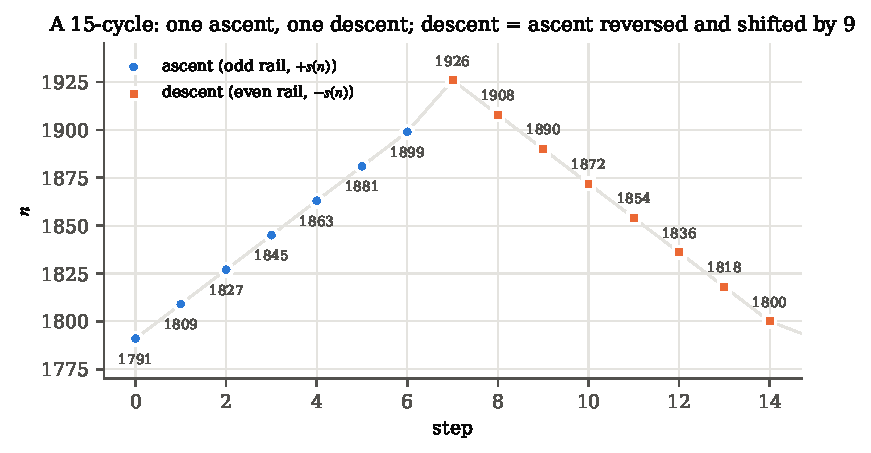
\includegraphics[width=0.92\textwidth]{figures/mountain_cycle.pdf}
\caption{The $15$-cycle through $1791$. Odd terms (circles) ascend by $18$
(once by $27$); even terms (squares) descend by $18$ (once by $9$). Here the
descent is the ascent run backwards and shifted by $+9$, as predicted by the
conditional reversibility identity (Theorem~\ref{thm:reverse}).}\label{fig:mountain}
\end{figure}

\paragraph{Main result.} Let $T(D)$ be the number of odd integers below $10^D$
that lie on a $2$-cycle.

\begin{theorem*}[Theorems~\ref{thm:2cycle}, \ref{thm:zero} and~\ref{thm:sharp}]
An odd $a$ lies on a $2$-cycle if and only if $s(a)$ is odd and
$a+s(a)$ produces exactly $s(s(a))/9$ carries. There are absolute constants
$c,K>0$ such that, for all sufficiently large $D$,
\[
  \frac{c}{\sqrt{\log D}}\le\frac{T(D)}{10^D}\le\frac{K}{\sqrt{\log D}} .
\]
\end{theorem*}

The mechanism is simple to state. The number of carries required for a
$2$-cycle is essentially its own mean (Theorem~\ref{thm:balance}); the carry
count is a sum of about $\log D$ weakly dependent terms; and such a sum hits a
value at its centre with probability of order $(\log D)^{-1/2}$.

\paragraph{Further results.}
\begin{itemize}
\item Self-similarity on multiples of nine and a digit formula for $s(9m)$
  (Theorem~\ref{thm:self}).
\item A general level equation describing how the digit sum changes under
  each step, and the resulting ``rail'' picture (Theorem~\ref{thm:level}).
\item A conditional time-reversal identity (Theorem~\ref{thm:reverse}); in the
  computed range, $43{,}194$ of the $43{,}210$ nonzero cycles have the ``mountain'' shape
  that it suggests. We do not prove a corresponding statement for all cycles.
\item Prefix lifting (Theorem~\ref{thm:lift}): an exact count of cycles
  confined to one prefix block, and a count of all cycles below $10^D$ with an
  explicit error of at most $18D\cdot10^{D-L}$ (Corollary~\ref{cor:lifterr}).
\item Carry resonance: an asymptotic formula for $T(D)/10^D$
  (Theorem~\ref{thm:resrig}); an exact formula for the variance of the carry
  count, $\frac{11}9\sum_i q_i(1-q_i)$ (Lemma~\ref{lem:exactvar}); a sharp local
  limit theorem for carries (Theorem~\ref{thm:sharpllt}); and the resulting
  \emph{oscillation law} (Theorem~\ref{thm:osclaw}): the normalised density
  $\sqrt{\log_{10}D}\,T(D)/10^D$ has no limit, its limit points fill an
  explicit interval, and $\limsup/\liminf=\sqrt{301}/11$
  (Corollary~\ref{cor:osc}).
\item A convergence criterion: an orbit is eventually periodic if and only if
  its digit sums are bounded (Theorem~\ref{thm:conv}); and every
  constant-level run moves an orbit by $O(k^2)$ (Theorem~\ref{thm:shortruns});
  and a computer-assisted proof that every orbit starting below $10^{2224}$
  (below $2^{3024}$ in base $2$) is eventually periodic
  (Theorems~\ref{thm:cert} and~\ref{thm:certres}).
  Global eventual periodicity (Conjecture~\ref{conj:conv}) remains open.
\item Other bases (Section~\ref{sec:bases}): in odd bases every orbit reaches
  $0$ (Theorem~\ref{thm:oddbase}); in every even base the structure theorems
  hold (Theorem~\ref{thm:evenbase}) and the $2$-cycle density is of exact order
  $(\log D)^{-1/2}$ (Theorem~\ref{thm:evenb}); in base $2$ this requires a
  different switch mechanism (Lemma~\ref{lem:binswitch}).
\end{itemize}

The main line of the paper is the density of $2$-cycles and its oscillation
(Sections~\ref{sec:resonance}--\ref{sec:balance}). The structural results
(Sections~3--7) supply the tools, and the other bases and convergence
(Sections~\ref{sec:bases} and~\ref{sec:convergence}) are further
applications. Figure~\ref{fig:deps} shows how the main results depend on
each other.

\begin{figure}[h]
\centering
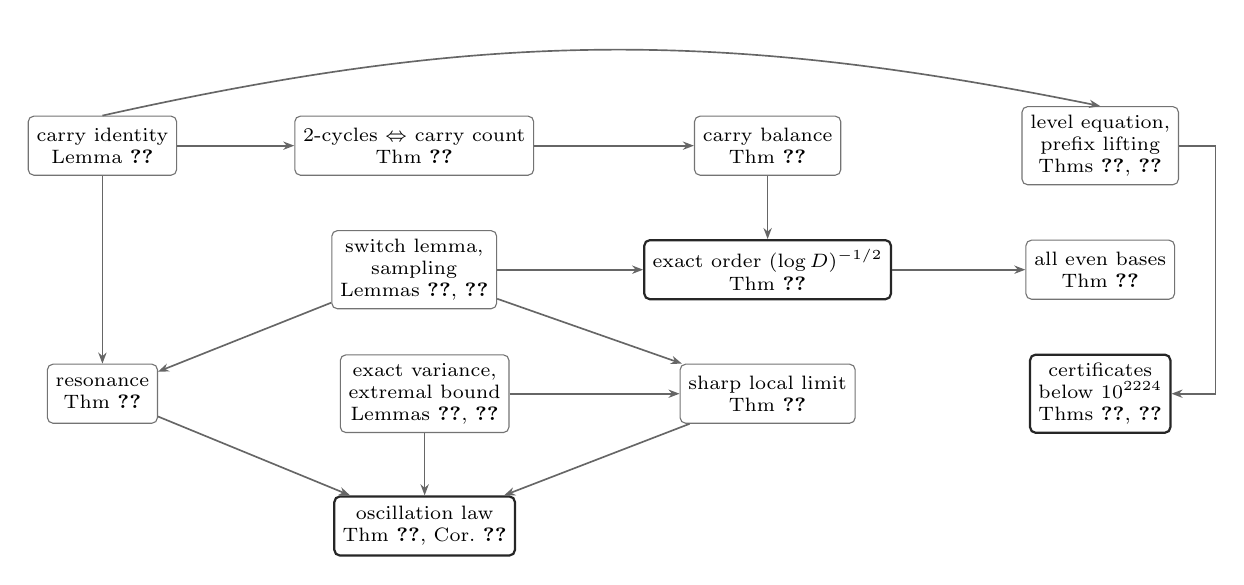
\begin{tikzpicture}[x=1.32cm,y=1.05cm,
  box/.style={draw=black!55, rounded corners=2pt, fill=white, font=\scriptsize, align=center, inner sep=3pt, minimum height=0.75cm},
  main/.style={box, draw=black!85, line width=0.8pt},
  arr/.style={-{Stealth[length=4pt]}, black!60, line width=0.6pt}]
\node[box]  (carry) at (0,0)     {carry identity\\ Lemma~\ref{lem:carry}};
\node[box]  (two)   at (3,0)     {$2$-cycles $\Leftrightarrow$ carry count\\ Thm~\ref{thm:2cycle}};
\node[box]  (bal)   at (6.4,0)   {carry balance\\ Thm~\ref{thm:balance}};
\node[box]  (sw)    at (3,-1.5)  {switch lemma,\\ sampling\\ Lemmas~\ref{lem:switch}, \ref{lem:sampling}};
\node[main] (sharp) at (6.4,-1.5){exact order $(\log D)^{-1/2}$\\ Thm~\ref{thm:sharp}};
\node[box]  (res)   at (0,-3)    {resonance\\ Thm~\ref{thm:resrig}};
\node[box]  (var)   at (3.1,-3)  {exact variance,\\ extremal bound\\ Lemmas~\ref{lem:exactvar}, \ref{lem:kappa}};
\node[box]  (llt)   at (6.4,-3)  {sharp local limit\\ Thm~\ref{thm:sharpllt}};
\node[main] (osc)   at (3.1,-4.6)  {oscillation law\\ Thm~\ref{thm:osclaw}, Cor.~\ref{cor:osc}};
\node[box]  (base)  at (9.6,-1.5){all even bases\\ Thm~\ref{thm:evenb}};
\node[box]  (lev)   at (9.6,0)   {level equation,\\ prefix lifting\\ Thms~\ref{thm:level}, \ref{thm:lift}};
\node[main] (cert)  at (9.6,-3)  {certificates\\ below $10^{2224}$\\ Thms~\ref{thm:cert}, \ref{thm:certres}};
\draw[arr] (carry) -- (two); \draw[arr] (two) -- (bal); \draw[arr] (bal) -- (sharp);
\draw[arr] (sw) -- (sharp); \draw[arr] (carry) -- (res); \draw[arr] (sw) -- (res);
\draw[arr] (res) -- (osc); \draw[arr] (var) -- (osc); \draw[arr] (llt) -- (osc);
\draw[arr] (var) -- (llt); \draw[arr] (sw) -- (llt); \draw[arr] (sharp) -- (base);
\draw[arr] (lev.east) -- ++(0.35,0) |- (cert.east); \draw[arr] (carry.north) to[bend left=12] (lev.north);
\end{tikzpicture}
\caption{Dependencies between the main results. Boxes with heavier frames are
the principal theorems.}\label{fig:deps}
\end{figure}

\section{Preliminaries}

Table~\ref{tab:notation} collects the notation used throughout.

\begin{table}[h]
\centering
\small
\begin{tabular}{>{\raggedright}p{2.9cm}>{\raggedright\arraybackslash}p{9.9cm}}
\toprule
symbol & meaning\\
\midrule
$s(n)$, $s_b(n)$ & digit sum of $n$ in base $10$, base $b$\\
$f$, $f_b$ & the digit-sum parity map~\eqref{eq:f} and its base-$b$ analogue\\
$\C(a,b)$, $\B(a,b)$ & number of carries in $a+b$, of borrows in $a-b$\\
$\C_K(a,t)$ & carries out of columns $0,\dots,K-1$ only\\
$k$, level & $s(n)=9k$ for a multiple of $9$; $\kappa(m)=s(9m)/9$\\
$T(D)$ & number of odd $a<10^D$ lying on a $2$-cycle\\
$P_D(t)$ & probability that $D$ uniform digits sum to $t$\\
$\rho(t)$ & probability that adding $t$ to a random odd number gives exactly $s(t)/9$ carries\\
$S(t)$, $W$ & switch positions of $t$ (Lemma~\ref{lem:switch}) and the random set of active switches\\
$q_i$, $\varphi$ & $q_i=\Pr(\text{carry into column }i)$; $\varphi(x)=x(1-x)$ (Section~\ref{sec:osclaw})\\
$h$, $B_D$, $K_0$ & scales and constants of the oscillation law (Theorem~\ref{thm:osclaw})\\
$H$, $L$, $\sigma$ & prefix and block length in $n=H10^L+x$; $\sigma=s(H)$\\
$g_\sigma$, $\bar g_\sigma$ & low map on $[0,b^L)$ and on the half-line (Section~\ref{sec:convergence})\\
$c_L(\sigma)$ & number of cycles of $g_\sigma$ confined to one block (Section~\ref{sec:lift})\\
\bottomrule
\end{tabular}
\caption{Notation.}\label{tab:notation}
\end{table}

All numbers are non-negative integers written in base $10$, with digits
$n=\sum_i n_i10^i$. For $a,b\ge0$ let $\C(a,b)$ be the number of carries in
the schoolbook addition $a+b$ (counting a final carry into a new leading
digit), and for $a\ge b\ge0$ let $\B(a,b)$ be the number of borrows in $a-b$.

\begin{lemma}[Carries and borrows]\label{lem:carry}
$s(a+b)=s(a)+s(b)-9\,\C(a,b)$, and for $a\ge b$,
$s(a-b)=s(a)-s(b)+9\,\B(a,b)$.
\end{lemma}

\begin{proof}
With incoming carries $c_i\in\{0,1\}$, $c_0=0$, column $i$ produces the digit
$a_i+b_i+c_i-10c_{i+1}$, and a final carry produces a leading digit equal to
it. Summing, $s(a+b)=s(a)+s(b)-9\sum_i c_{i+1}=s(a)+s(b)-9\C(a,b)$. The
second identity is the first applied to $(a-b)+b=a$, whose carries are the
borrows of $a-b$.
\end{proof}

This is the base-$10$ form of the identity behind Kummer's theorem on
carries~\cite{Kummer}; the statistics of carries are studied
in~\cite{Holte,DiaconisFulman}.

\begin{lemma}\label{lem:mod9}
$s(n)\equiv n\pmod9$; hence $9\mid f(n)$ for even $n$, and $9\mid n$
implies $9\mid f(n)$.
\end{lemma}

\begin{proof}
Since $10\equiv1\pmod9$, $n=\sum_in_i10^i\equiv\sum_in_i=s(n)\pmod9$. For even
$n$, $f(n)=n-s(n)\equiv0\pmod9$. If $9\mid n$ then $9\mid s(n)$, so
$9\mid n\pm s(n)=f(n)$.
\end{proof}

\begin{proposition}[Reduction to multiples of nine]\label{prop:nine}
Every term after the first even term of an orbit is a multiple of $9$. The
first even term may come late: $11\to13\to17\to25\to32\to27$ needs five steps
to reach a multiple of $9$, and among $n<10^6$ the maximum is $14$ steps
(at $n=899457$).
\end{proposition}

\begin{proof}
If $m$ is even then $9\mid f(m)$ by Lemma~\ref{lem:mod9}, and by the same lemma
every later term is again a multiple of $9$, by induction. The statements about
$11$ and about $n<10^6$ are computational: they were obtained by iterating $f$
from every starting value (see the Data and code section).
\end{proof}

\begin{remark}
In particular, an orbit need not reach a multiple of nine within two steps,
and an odd multiple of $9$ need not map to an even number: if its digit sum
is even it stays odd, and this is exactly what produces the ascending runs of
Section~\ref{sec:rails}.
\end{remark}

\section{Self-similarity and a digit formula for $s(9m)$}

\begin{theorem}[Self-similarity]\label{thm:self}
For $m\ge0$ let $\kappa(m)=s(9m)/9$. Then
\[
  \kappa(m)\;=\;\B(10m,m)\;=\;\#\bigl\{\,i\ge0:\ m_i>9\cdot 0.m_{i-1}m_{i-2}\cdots m_0\,\bigr\},
\]
where $0.m_{i-1}\cdots m_0$ is the number in $[0,1)$ formed by the digits
below position $i$ (empty for $i=0$). Moreover $9m\mapsto f(9m)$ is conjugate
to
\[
  g(m)=\begin{cases} m+\kappa(m), & m\text{ odd},\\ m-\kappa(m), & m\text{ even}.\end{cases}
\]
\end{theorem}

\begin{proof}
Since $9m=10m-m$ and $s(10m)=s(m)$, Lemma~\ref{lem:carry} gives
$s(9m)=s(10m)-s(m)+9\B(10m,m)=9\B(10m,m)$. In a subtraction $a-b$ a borrow
leaves column $i$ exactly when $a\bmod10^{i+1}<b\bmod10^{i+1}$. With $a=10m$,
$a\bmod10^{i+1}=10\,(m\bmod10^i)$, and the condition
$10(m\bmod10^i)<m_i10^i+(m\bmod10^i)$ is $m_i>9(m\bmod10^i)/10^i$. Finally
$9m$ and $m$ have the same parity, so $f(9m)=9m\pm s(9m)=9\,g(m)$.
\end{proof}

For instance $\kappa(11)=2$: $m_0=1>0$ and $m_1=1>9\cdot0.1$; indeed
$s(99)=18$. The theorem was checked against direct computation for all
$m<10^6$.

\section{Rails and the level equation}\label{sec:rails}

\begin{definition}
On multiples of $9$ write $s(n)=9k$ and call $k$ the \emph{level} of $n$.
The \emph{odd rail} consists of the odd multiples of $9$ and the \emph{even
rail} of the even ones.
\end{definition}

\begin{theorem}[Level equation]\label{thm:level}
Let $9\mid n$ with level $k$, i.e.\ $s(n)=9k$, and let $\kappa(k)=s(9k)/9$ as
in Theorem~\ref{thm:self}. Then
\[
  s(n+9k)=9\bigl(k+\kappa(k)-\C(n,9k)\bigr),\qquad
  s(n-9k)=9\bigl(k-\kappa(k)+\B(n,9k)\bigr)\quad(n\ge9k).
\]
Thus an ascending step keeps the level if and only if it produces exactly
$\kappa(k)$ carries, and a descending step keeps the level if and only if it
produces exactly $\kappa(k)$ borrows. A step keeps the rail (the parity of
$n$) if and only if $k$ is even. In particular, for $1\le k\le10$ one has
$\kappa(k)=1$, so the level is kept exactly when there is one carry or one
borrow.
\end{theorem}

\begin{proof}
By Lemma~\ref{lem:carry}, $s(n\pm9k)=s(n)\pm s(9k)\mp9\,\C$ (resp.\ $\pm9\B$),
and $s(9k)=9\kappa(k)$. The parity of $n\pm9k$ equals that of $n$ iff $9k$ is
even, i.e.\ $k$ is even. For $1\le k\le10$, $9k\in\{9,18,\dots,90\}$ has digit
sum $9$.
\end{proof}

The general form matters because a typical $D$-digit multiple of $9$ has level
$k\approx D/2$, far beyond $10$ when $D$ is large; the equation was checked on
$20{,}000$ random multiples of $9$ with up to $60$ digits, $13{,}315$ of them
with $k>10$. Theorem~\ref{thm:level} explains the regular motion seen in
Figure~\ref{fig:mountain}: for small $k$, adding $9k=10k-k$ typically lowers
the units digit by $k$ and raises the tens digit by $k$, leaving the digit sum
and hence the step size unchanged. In general the orbit is a translation along
its rail as long as each step produces exactly $\kappa(k)$ carries or borrows;
an \emph{exceptional} step, with a different number, changes the level.
Figure~\ref{fig:rails} summarises the resulting picture.

\begin{figure}[t]
\centering
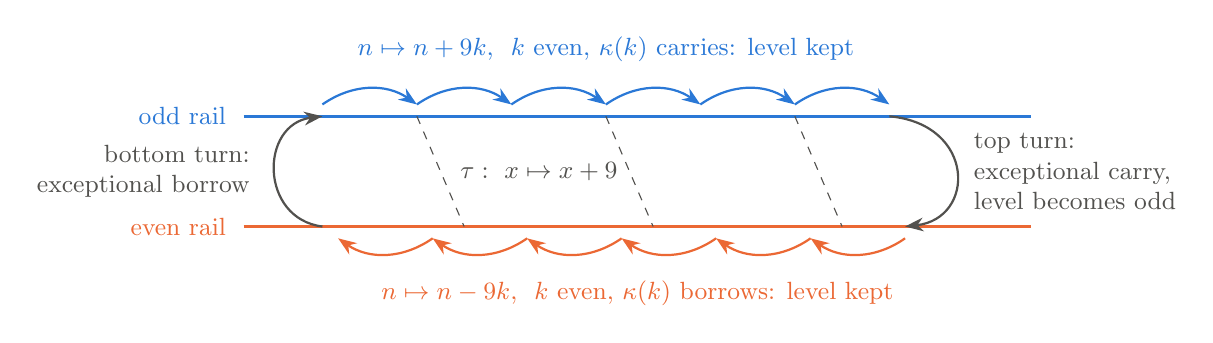
\begin{tikzpicture}[>=Stealth, every node/.style={font=\small}]
  \draw[rail1, line width=1.2pt] (0,1.4) -- (10,1.4);
  \draw[rail2, line width=1.2pt] (0,0) -- (10,0);
  \node[rail1, anchor=east] at (-0.1,1.4) {odd rail};
  \node[rail2, anchor=east] at (-0.1,0) {even rail};
  \foreach \x in {1,2.2,3.4,4.6,5.8,7.0} {
    \draw[->, rail1, thick] (\x,1.55) to[bend left=35] (\x+1.2,1.55);
  }
  \node[rail1] at (4.6,2.25) {$n\mapsto n+9k$, \ $k$ even, $\kappa(k)$ carries: level kept};
  \foreach \x in {8.4,7.2,6.0,4.8,3.6,2.4} {
    \draw[->, rail2, thick] (\x,-0.15) to[bend left=35] (\x-1.2,-0.15);
  }
  \node[rail2] at (5.0,-0.85) {$n\mapsto n-9k$, \ $k$ even, $\kappa(k)$ borrows: level kept};
  \draw[->, thick, ink2] (8.2,1.4) .. controls (9.3,1.3) and (9.3,0.1) .. (8.4,0.0);
  \node[ink2, align=left, anchor=west] at (9.15,0.7) {top turn:\\ exceptional carry,\\ level becomes odd};
  \draw[->, thick, ink2] (1.0,0.0) .. controls (0.2,0.1) and (0.2,1.3) .. (1.0,1.4);
  \node[ink2, align=right, anchor=east] at (0.2,0.7) {bottom turn:\\ exceptional borrow};
  \foreach \x in {2.2,4.6,7.0} {
    \draw[dashed, ink2] (\x,1.4) -- (\x+0.6,0);
  }
  \node[ink2, fill=white, inner sep=1.5pt] at (3.75,0.7) {$\tau:\ x\mapsto x+9$};
\end{tikzpicture}
\caption{Rails and turns. Regular steps translate along a rail; the shift
$\tau$ maps the odd rail to the even rail and reverses time
(Theorem~\ref{thm:reverse}), so the descent retraces the ascent.}\label{fig:rails}
\end{figure}

\section{A conditional time-reversal identity and mountain cycles}

\begin{theorem}[Conditional reversibility]\label{thm:reverse}
Let $x\ge0$. If $s(x)$ is even and $s(f(x)+9)=s(x)$, then
\[
  f\bigl(f(x)+9\bigr)=x+9 .
\]
Equivalently, writing $\tau(x)=x+9$, we have $f(\tau(f(x)))=\tau(x)$ at every
such $x$. This is a conditional identity, not a global symmetry: it says
nothing about points where either hypothesis fails.
\end{theorem}

\begin{proof}
Let $S=s(x)$, even. If $x$ is odd, $f(x)=x+S$ is odd and $y=x+S+9$ is even,
so $f(y)=y-s(y)=x+S+9-S=x+9$. If $x$ is even, $f(x)=x-S$ is even and
$y=x-S+9$ is odd, so $f(y)=y+s(y)=x+9$.
\end{proof}

When the hypotheses hold along a whole stretch of an orbit, the stretch is
retraced, shifted by $9$, in the opposite direction. They hold on
\emph{regular} stretches: by Lemma~\ref{lem:carry},
$s(f(x)+9)=s(f(x))+9-9\C(f(x),9)$, which equals $s(f(x))$ exactly when adding
$9$ to $f(x)$ produces one carry, while $s(f(x))=s(x)$ on a level-preserving
step (Theorem~\ref{thm:level}). The identity was also checked directly for all
$31{,}196$ applicable $x<10^6$.

This suggests the \emph{mountain} shape seen in Figure~\ref{fig:mountain}: an
ascent on the odd rail, a turn, a descent on the even rail that is the
$\tau$-image of the ascent run backwards, and a second turn that closes the
loop. We record its prevalence as a computational statement only.

\begin{proposition}[Computational census]\label{prop:census}
Of the $43{,}210$ distinct cycles other than the fixed point $\{0\}$ reached
from the starting values $1\le n\le2\cdot10^6$ (the fixed point $0$, reached
for instance by $1\to2\to0$, brings the total to $43{,}211$), exactly $43{,}194$ consist of one ascending run (odd
terms) followed by one descending run (even terms); the other $16$ have two
ascending and two descending runs, the smallest being
$799020\to798993\to799038\to799002\to798975$.
\end{proposition}

We do not know whether almost all cycles of $f$, in the sense of density, have
the mountain shape; Theorem~\ref{thm:reverse} gives a mechanism for it but not
a proof. A $2$-cycle is a mountain without regular stretches.

\section{Two-cycles}

\begin{proposition}[Two-step identity]\label{prop:twostep}
If $n$ and $s(n)$ are odd, then $f(n)$ is even and
$f^2(n)=n-s(s(n))+9\,\C(n,s(n))$.
\end{proposition}

\begin{proof}
By Lemma~\ref{lem:carry}, $s(f(n))=s(n)+s(s(n))-9\C(n,s(n))$, and
$f^2(n)=n+s(n)-s(f(n))$.
\end{proof}

\begin{theorem}[Characterisation of $2$-cycles]\label{thm:2cycle}
Every $2$-cycle $\{a,b\}$, $a\ne b$, contains exactly one odd number, and an
odd $a$ lies on a $2$-cycle if and only if $s(a)$ is odd and
$s(s(a))=9\,\C(a,s(a))$. Then $9\mid a$; and if $a<10^{11}-1$ the condition
reads: $s(a)$ is odd and $a+s(a)$ has exactly one carry.
\end{theorem}

\begin{proof}
Two even (or two odd) points would give $b<a<b$. For odd $a$, $b=a+s(a)$
must be even (else $f(b)>b>a$), so $s(a)$ is odd, and $f(b)=a$ is
$f^2(a)=a$, i.e.\ $s(s(a))=9\C(a,s(a))$ by Proposition~\ref{prop:twostep}. The
converse is immediate. Since $s(s(a))\equiv a\pmod 9$, $9\mid a$. For
$a<10^{11}-1$, $s(a)\le98$, so $s(a)\in\{9,27,45,63,81\}$, each with digit
sum $9$.
\end{proof}

\begin{example}
$27+9=36$ has one carry, so $\{27,36\}$ is a $2$-cycle. $999+27=1026$ has three,
so $999$ is not on a $2$-cycle: $f(1026)=1017$.
\end{example}

Let $T(D)$ be the number of odd $a<10^D$ on a $2$-cycle. By
Theorem~\ref{thm:2cycle}, $T(D)$ is computed exactly by a digit-by-digit
dynamic programme over (carry, digit sum so far, carries so far), summing over
admissible $t=s(a)\equiv9\pmod{18}$; it agrees with exhaustive enumeration for
$D\le5$. Values are given in Table~\ref{tab:density}.

\section{Prefix lifting}\label{sec:lift}

\begin{figure}[t]
\centering
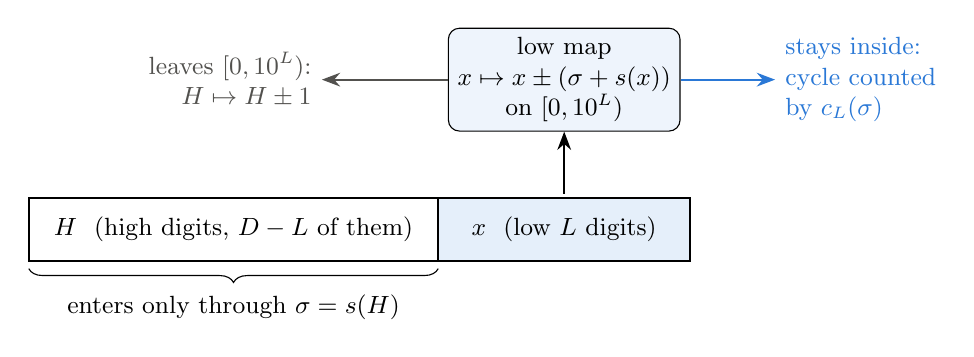
\begin{tikzpicture}[>=Stealth, every node/.style={font=\small}]
  \draw[thick] (0,0) rectangle (5.2,0.8);
  \draw[thick, fill=rail1!12] (5.2,0) rectangle (8.4,0.8);
  \node at (2.6,0.4) {$H$ \ (high digits, $D-L$ of them)};
  \node at (6.8,0.4) {$x$ \ (low $L$ digits)};
  \draw[decorate,decoration={brace,amplitude=5pt,mirror}] (0,-0.1) -- (5.2,-0.1)
     node[midway,below=6pt] {enters only through $\sigma=s(H)$};
  \node[draw, rounded corners, align=center, fill=rail1!8] (low) at (6.8,2.3)
     {low map\\ $x\mapsto x\pm(\sigma+s(x))$\\ on $[0,10^L)$};
  \draw[->, thick] (6.8,0.85) -- (low.south);
  \draw[->, thick, ink2] (low.west) -- ++(-1.6,0) node[left, align=right] {leaves $[0,10^L)$:\\ $H\mapsto H\pm1$};
  \draw[->, thick, rail1] (low.east) -- ++(1.2,0) node[right, align=left] {stays inside:\\ cycle counted\\ by $c_L(\sigma)$};
\end{tikzpicture}
\caption{Prefix lifting. Since $s(n)=s(H)+s(x)$ and $n$ has the parity of $x$,
the orbit of $H\cdot10^L+x$ depends on $H$ only through $\sigma=s(H)$ until
the prefix changes.}\label{fig:lift}
\end{figure}

\begin{theorem}[Prefix lifting]\label{thm:lift}
Fix $L\ge1$ and for $\sigma\ge0$ let $g_\sigma(x)=x+\sigma+s(x)$ for odd $x$
and $x-\sigma-s(x)$ for even $x$. Let $c_L(\sigma)$ be the number of cycles of
$g_\sigma$ contained in $[0,10^L)$. Then for every prefix $H$ the cycles of
$f$ all of whose terms have the form $H\cdot10^L+x$ with $0\le x<10^L$
correspond bijectively to these cycles of $g_{s(H)}$. Consequently the number
of cycles of $f$ below $10^D$ whose terms share a common prefix (above the
last $L$ digits) is
\[
  \sum_{\sigma\ge0} c_L(\sigma)\, N(D-L,\sigma),\qquad
  N(d,\sigma)=[z^\sigma]\Bigl(\frac{1-z^{10}}{1-z}\Bigr)^{d},
\]
where $N(d,\sigma)$ counts $d$-digit strings (leading zeros allowed) with
digit sum $\sigma$. The same holds for cycles of any fixed length.
\end{theorem}

\begin{proof}
For $n=H\cdot10^L+x$ with $0\le x<10^L$ we have $s(n)=s(H)+s(x)$, and
$n\equiv x\pmod2$. So as long as $g_{s(H)}(x)\in[0,10^L)$,
$f(n)=H\cdot10^L+g_{s(H)}(x)$. A cycle of $f$ with constant prefix $H$ is
therefore a cycle of $g_{s(H)}$ inside $[0,10^L)$, and conversely. Summing
over prefixes $H<10^{D-L}$ grouped by $s(H)$ gives the formula.
\end{proof}

Theorem~\ref{thm:lift} counts only cycles confined to one prefix block. The
remaining cycles cross a block boundary, and they are few.

\begin{corollary}[Counting all cycles, with error bound]\label{cor:lifterr}
Let $Z(D)$ be the number of cycles of $f$ all of whose terms are below $10^D$
(including the fixed point $0$), and let $Z_L(D)=\sum_\sigma
c_L(\sigma)N(D-L,\sigma)$. If $9D<10^L$, then
\[
  Z_L(D)\;\le\;Z(D)\;\le\;Z_L(D)+18D\cdot10^{D-L}.
\]
The same bound holds for cycles of any fixed length, in particular for
$2$-cycles.
\end{corollary}

\begin{proof}
Every cycle counted by $Z_L(D)$ is counted by $Z(D)$. A cycle not counted by
$Z_L(D)$ has terms in at least two prefix blocks, so it contains a term $n$
with $f(n)$ in a different block. Since $|f(n)-n|=s(n)\le9D<10^L$, the low
part $x=n\bmod10^L$ then satisfies $x\ge10^L-9D$ (if $f(n)>n$) or $x<9D$ (if
$f(n)<n$). At most $2\cdot9D\cdot10^{D-L}$ integers below $10^D$ have such a
low part, and distinct cycles are disjoint.
\end{proof}

\paragraph{Algorithm.} Compute $c_L(\sigma)$ for all needed $\sigma$ (a
functional graph on $10^L$ vertices per $\sigma$, with cycles found by pointer
doubling), then evaluate the polynomial coefficients. This costs
$O(10^L\cdot L\cdot\sigma_{\max}+D\,\sigma_{\max})$ with $\sigma_{\max}\le9D$,
instead of the $10^D$ orbits of brute force, and by
Corollary~\ref{cor:lifterr} it determines $Z(D)/10^D$ to within $18D/10^L$.
Choosing $L$ a little larger than $\log_{10}D$ therefore makes the relative
error as small as desired. For example, for $D=200$ the guaranteed error in
$Z(D)/10^D$ is $0.36$ with $L=4$, $0.036$ with $L=5$ and $0.0036$ with $L=6$.
The profile costs about $10^L\cdot L$ operations for each of the
$\sigma_{\max}\approx1{,}800$ values of $\sigma$, i.e.\ about $10^9$ operations
for $L=5$; in our implementation the $L=5$ profile (for all
$\sigma\le2{,}500$) took under a minute on a laptop, and each extra digit of
$L$ multiplies the cost by about $10$. In practice the agreement is much better than this
bound: with $L=3$ the formula reproduces the brute-force counts $2026$ ($D=5$)
and $21566$ ($D=6$) exactly, and with $L=5$, restricted to $2$-cycles, it
reproduces the exact $T(D)/10^D$ to six decimal places for every
$6\le D\le200$ in Table~\ref{tab:density} (where the bound
$18D/10^L$ alone would only guarantee about two decimal places).

The profile $c_2(\sigma)$ (Figure~\ref{fig:profile}) is irregular, and that
is the source of every oscillation in the counts: the density of cycles below
$10^D$ is the average of $c_L(\sigma)/10^L$ against the digit-sum
distribution of a random $(D-L)$-digit prefix, a bell curve centred at
$4.5(D-L)$ of width about $\sqrt{8.25D}$, which slides across the
irregularities as $D$ grows.

\begin{figure}[t]
\centering
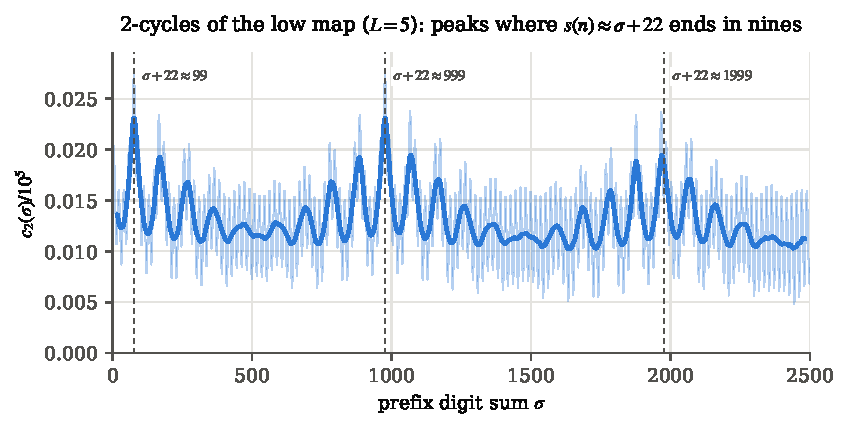
\includegraphics[width=0.92\textwidth]{figures/profile_c2.pdf}
\caption{Number of $2$-cycles of the low map $g_\sigma$ for $L=5$ (thin) and
an $18$-term moving average (thick). Peaks occur where the typical digit sum
$s(n)\approx\sigma+22$ ends in a run of nines.}\label{fig:profile}
\end{figure}

\section{Carry resonance and the density of $2$-cycles}\label{sec:resonance}

For an odd multiple $t$ of $9$ let $\rho(t)$ be the probability that adding
$t$ to a random integer with odd units digit produces exactly $s(t)/9$
carries. With a uniformly random digit of $a$, a column whose digit of $t$ is
$d$ and whose incoming carry is $c$ produces a carry with probability
$(d+c)/10$. Hence, marking carries by $z$,
\[
  \rho(t)=[z^{s(t)/9}]\; u^{\top}\,M_1(t_0)\,M(t_1)\cdots M(t_{\ell-1})\,M(0)^{\infty}\,\mathbf 1,
  \qquad
  M(d)=\frac1{10}\begin{pmatrix}10-d & d\,z\\ 9-d & (d+1)\,z\end{pmatrix},
\]
with $u=(1,0)^\top$ and $M_1$ the units column restricted to odd digits.
This is the carries Markov chain~\cite{Holte,DiaconisFulman}.

\begin{proposition}\label{prop:resonance}
$\rho(10^j-1)=9/10$ for every $j\ge1$.
\end{proposition}

\begin{proof}
Adding $t=10^j-1$ to $a$ with odd units digit: the units column gives
$a_0+9\ge10$, and each of the next $j-1$ columns gives $a_i+9+1\ge10$, so all
$j$ columns carry and $s(t)/9=j$. Exactly $j$ carries occur iff column $j$
does not carry, i.e.\ $a_j\ne9$, which has probability $9/10$.
\end{proof}

When $t$ consists of nines the required number of carries is forced; when $t$
has small or mixed digits, matching it is a coin flip (for example
$\rho(45)=\rho(63)=0.444$). Figure~\ref{fig:rho} shows the resulting
\emph{carry resonance}.

\begin{figure}[t]
\centering
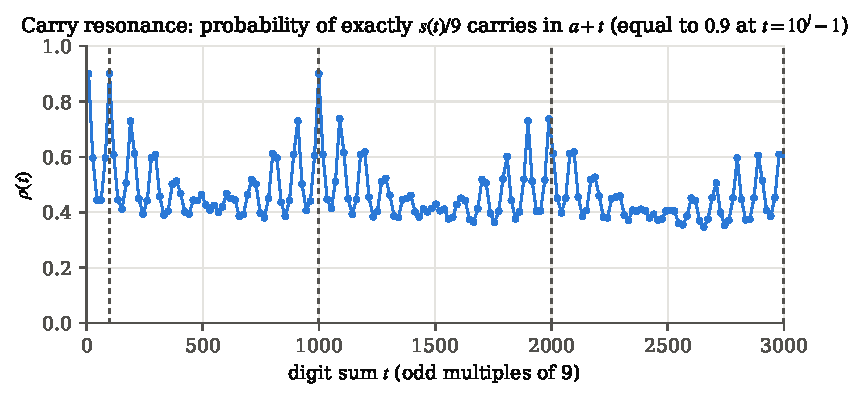
\includegraphics[width=0.92\textwidth]{figures/carry_resonance.pdf}
\caption{$\rho(t)$ for odd multiples $t$ of $9$. The maximum $9/10$ is attained
at $t=10^j-1$ (Proposition~\ref{prop:resonance}).}\label{fig:rho}
\end{figure}

Treating $s(a)=t$, the parity of $a$ and the carries as independent gives
the \emph{resonance approximation}
\[
  \frac{T(D)}{10^D}\;\approx\;\frac12\sum_{t\equiv 9\ (18)} P_D(t)\,\rho(t),
\]
where $P_D(t)$ is the probability that a random $D$-digit string has digit sum
$t$. Table~\ref{tab:density} compares it with the exact values: the error is
below $10^{-4}$ for $12\le D\le200$ and below $2\cdot10^{-6}$ for
$100\le D\le200$.

\begin{table}[t]
\centering
\begin{tabular}{rcc@{\qquad}rcc}
\toprule
$D$ & exact & resonance & $D$ & exact & resonance\\
\midrule
6 & 0.018879 & 0.017810 & 30 & 0.013760 & 0.013711\\
8 & 0.013812 & 0.014153 & 50 & 0.013827 & 0.013807\\
10 & 0.013101 & 0.012902 & 75 & 0.012426 & 0.012412\\
12 & 0.012434 & 0.012450 & 100 & 0.011919 & 0.011919\\
15 & 0.013855 & 0.013795 & 150 & 0.012165 & 0.012163\\
20 & 0.019908 & 0.019996 & 200 & 0.014819 & 0.014821\\
\bottomrule
\end{tabular}
\caption{Proportion $T(D)/10^D$ of integers below $10^D$ that are the odd point
of a $2$-cycle: exact (digit dynamic programme) and resonance approximation.}
\label{tab:density}
\end{table}

Since $s(a)$ concentrates near $4.5D$, the density peaks when $4.5D$ lies just
below a power of ten (the relevant $t$ end in nines) and dips in between.
Evaluating the approximation up to $D=10^4$ (Figure~\ref{fig:density}) gives
peaks near $D=22,\,218,\,2247$ with heights $0.0210,\,0.0160,\,0.0145$, and
troughs near $D=554$ and $5452$ with values $0.0109$ and $0.0098$; at
$D=10^4$ the density is about $0.0096$.

\begin{figure}[t]
\centering
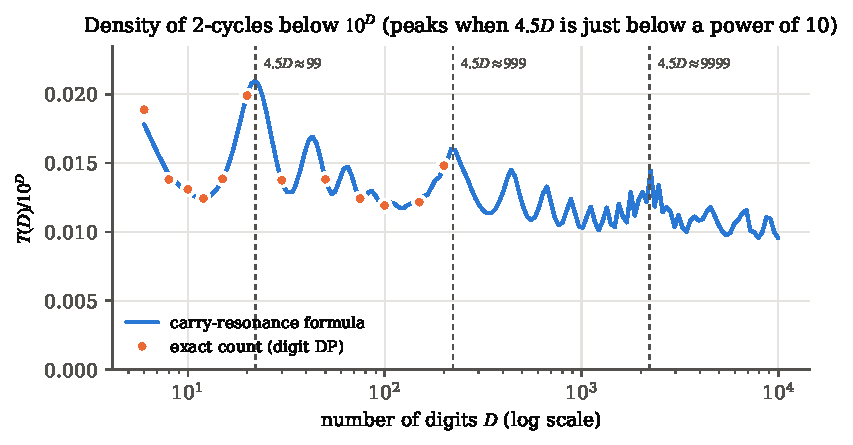
\includegraphics[width=0.92\textwidth]{figures/density_2cycles.pdf}
\caption{Density of $2$-cycles below $10^D$: exact values (dots) and the
resonance approximation (line), with $4.5D=99,999,9999$ marked.}\label{fig:density}
\end{figure}

Figure~\ref{fig:density} suggests that the normalised density
$\sqrt{\log_{10}D}\,T(D)/10^D$ has no limit, with local maxima near
$D\approx(10^j-1)/4.5$. Corollary~\ref{cor:osc} in Section~\ref{sec:osclaw}
proves this and identifies the limit points exactly: the ratio
$\limsup/\liminf$ equals $\sqrt{301}/11\approx1.577$. Table~\ref{tab:osc}
illustrates how slowly this limit is approached.

By Theorem~\ref{thm:resrig}, the oscillation concerns only the main term
$\tfrac12\sum_tP_D(t)\rho(t)$, since its error $O((\log D)^2/\sqrt D)$ is much
smaller than the main term, which is of order $(\log D)^{-1/2}$. We evaluated
the main term with a Gaussian approximation to $P_D$ (which agrees with the
exact convolution to six decimal places at $D=200,1000,5000$) up to
$D\approx6\cdot10^7$. Table~\ref{tab:osc} shows that over six orders of
magnitude of $D$ the ratio between consecutive local maxima and minima stays
between $1.375$ and $1.413$, still well below its limit $1.577$; Remark~\ref{rem:slow}
explains why.

\begin{table}[h]
\centering
\begin{tabular}{rrcrcc}
\toprule
$j$ & peak at $D$ & normalised peak & trough at $D$ & normalised trough & ratio\\
\midrule
3 & 222 & 0.02482 & 777 & 0.01781 & 1.394\\
4 & 2{,}222 & 0.02720 & 7{,}777 & 0.01942 & 1.401\\
5 & 22{,}222 & 0.02753 & 38{,}888 & 0.02001 & 1.375\\
6 & 222{,}222 & 0.02891 & 614{,}035 & 0.02072 & 1.395\\
7 & 2{,}222{,}222 & 0.02904 & 6{,}345{,}029 & 0.02082 & 1.394\\
8 & 22{,}222{,}222 & 0.02995 & 63{,}450{,}292 & 0.02120 & 1.413\\
\bottomrule
\end{tabular}
\caption{Local maxima and minima of $\sqrt{\log_{10}D}\,\cdot\frac12\sum_tP_D(t)\rho(t)$,
the normalisation of Corollary~\ref{cor:osc}, whose limits are
$K_0\sqrt6\approx0.0347$ and $K_0\sqrt{726/301}\approx0.0220$
(computational; the extrema were located by a search over a grid of $D$ near
$(10^j-1)/4.5$ and $2.5\cdot10^j/4.5$).}\label{tab:osc}
\end{table}

The mechanism is the one behind Proposition~\ref{prop:resonance}. The digit
sum $t$ of a random $D$-digit number lies within $O(\sqrt D)$ of $4.5D$, so its
top $\approx\frac12\log_{10}D$ digits are determined by $D$ and only its bottom
digits vary. When $4.5D$ is just below $10^j$, those top digits are nines;
columns of $a+t$ where $t$ has a nine carry almost deterministically, so only
the bottom half of the columns contributes to the variance of the carry
count, and the probability of hitting its mean is correspondingly larger. At
other values of $D$ all columns contribute. Section~\ref{sec:osclaw} makes this precise. The variance of the carry
count equals $\frac{11}9\sum_i\varphi(q_i)$ exactly (Lemma~\ref{lem:exactvar}),
and a sharp local limit theorem (Theorem~\ref{thm:sharpllt}) turns it into the
oscillation law, Theorem~\ref{thm:osclaw}.

\section{Two-cycles have density zero}\label{sec:zero}

Throughout this section $K,K_0,K_1,\dots$ denote absolute constants and
$c>0$ an absolute constant, not necessarily the same at each occurrence. For
an integer $t\ge1$ with digits $t_i$ let
\[
  S(t)=\bigl\{\,i\ \text{odd},\ i\ge1:\ t_i\in\{1,\dots,8\}\,\bigr\}.
\]
For a random variable $X$ and $\lambda>0$, $Q(X;\lambda)=\sup_x
\Pr(x\le X\le x+\lambda)$ is its concentration function. We use the
Kolmogorov--Rogozin inequality~\cite{Rogozin,Petrov}: for independent
$X_1,\dots,X_n$ and $0<\lambda\le L$,
\begin{equation}\label{eq:KR}
  Q\Bigl(\sum_i X_i;L\Bigr)\le K_0\,L\Bigl(\sum_i\lambda^2\bigl(1-Q(X_i;\lambda)\bigr)\Bigr)^{-1/2}.
\end{equation}
For integer-valued variables and $\lambda=L=\tfrac12$, $Q(X;\tfrac12)$ is the
largest point probability, so~\eqref{eq:KR} gives
$\max_m\Pr(\sum_iX_i=m)\le K_0\bigl(\sum_i(1-\max_x\Pr(X_i=x))\bigr)^{-1/2}$.

\begin{lemma}[Switch lemma]\label{lem:switch}
Let $t\ge1$ have $\ell$ digits, let $0<\delta\le\tfrac1{10}$, and let
$a=\sum_i a_i10^i$ have independent digits $a_0,a_1,\dots$ such that
$\Pr(a_i=d)\ge\delta$ for all $d\in\{0,\dots,9\}$ and $1\le i\le\ell$. Let
$C$ be the number of carries in $a+t$, possibly counting only the carries out
of columns $0,\dots,k-1$ for some fixed $k>\ell$. Then for every integer $m$
\[
  \Pr(C=m)\;\le\;\frac{K_1}{\delta\sqrt{|S(t)|}}+e^{-9\delta|S(t)|/8}.
\]
\end{lemma}

\begin{proof}
Write $c_j$ for the carry into column $j$. For $i\in S(t)$ call $i$ a
\emph{switch} if $a_{i+1}+t_{i+1}\neq9$, and let $W$ be the set of switches.
Since $i+1$ is even, $W$ depends only on the digits at even positions, and
the events $\{i\in W\}$, $i\in S(t)$, are independent with
$\Pr(i\in W)=1-\Pr(a_{i+1}=9-t_{i+1})\ge9\delta$.

Condition on $G=(a_j)_{j\notin W}$, which determines $W$; the digits
$a_i$, $i\in W$, remain independent with their original laws. We claim that
\begin{equation}\label{eq:switchsum}
  C=C_0+\sum_{i\in W}\xi_i,\qquad \xi_i=\mathbf 1\{a_i\ge\theta_i\},
\end{equation}
where $C_0$ and $\theta_i\in\{1,\dots,9\}$ are functions of $G$. Indeed, for
$i\in W$ the carry $c_{i+2}=\mathbf1\{a_{i+1}+t_{i+1}+c_{i+1}\ge10\}$ equals
$\mathbf1\{a_{i+1}+t_{i+1}\ge10\}$, because $a_{i+1}+t_{i+1}\ne9$; so the value
of $a_i$ influences no carry other than $c_{i+1}$. Proceeding upwards through
the columns, every carry $c_j$ with $j\notin\{i+1:i\in W\}$ is therefore a
function of $G$. In particular, for $i\in W$ the carry $c_i$ into column $i$
is a function of $G$ (as $i-1$ is even, $i\neq i'+1$ for $i'\in W$), and
$c_{i+1}=\mathbf1\{a_i\ge\theta_i\}$ with $\theta_i=10-t_i-c_i$. Since
$t_i\in\{1,\dots,8\}$, $\theta_i\in\{1,\dots,9\}$, which proves the claim;
truncating the count at column $k-1$ only changes $C_0$.

Given $G$, each $\xi_i$ is Bernoulli with
$\Pr(\xi_i=1\mid G)=\Pr(a_i\ge\theta_i)\in[\delta,1-\delta]$, so
$1-\max_x\Pr(\xi_i=x\mid G)\ge\delta$. By~\eqref{eq:KR},
$\Pr(C=m\mid G)\le K_0(\delta|W|)^{-1/2}$. By the multiplicative Chernoff
bound~\cite[Thm.~4.5]{MitzenmacherUpfal}, $\Pr(|W|<\tfrac92\delta|S(t)|)\le e^{-9\delta|S(t)|/8}$.
On the complementary event,
$\Pr(C=m\mid G)\le K_0(\tfrac92\delta^2|S(t)|)^{-1/2}$, and the lemma follows.
\end{proof}

\begin{lemma}[Sampling]\label{lem:sampling}
Let $x_0,\dots,x_{D-1}$ be a uniformly random arrangement of a multiset of $D$
digits with counts $N_0,\dots,N_9$, and let $y_0,y_1,\dots$ be independent
with $\Pr(y_i=d)=N_d/D$. For $k\le D$, the laws of $(x_0,\dots,x_{k-1})$ and
$(y_0,\dots,y_{k-1})$ are within total variation distance $k(k-1)/(2D)$.
\end{lemma}

\begin{proof}
Realise both by drawing balls from an urn of $D$ labelled balls, without and
with replacement. The two procedures can be coupled to agree unless a ball is
drawn twice with replacement, which has probability at most
$\binom k2/D$~\cite{DiaconisFreedman}.
\end{proof}

\begin{lemma}[Low digits of the digit sum]\label{lem:lowdigits}
Let $a$ be uniform in $\{0,\dots,10^D-1\}$ and $t=s(a)$. There is $K_2$ such
that for every modulus $M\ge1$ the law of $t\bmod M$ is within total
variation distance $K_2\,M/\sqrt D$ of the uniform law on
$\{0,\dots,M-1\}$. (We use $M=10^h$ and $M=9\cdot10^h$.)
\end{lemma}

\begin{proof}
The law of $t$ is the $D$-fold convolution of the uniform law on
$\{0,\dots,9\}$. Convolutions of log-concave sequences are
log-concave~\cite{Hoggar}, so it is unimodal, and by~\eqref{eq:KR} its largest
point probability is $p_{\max}\le K/\sqrt D$. For a unimodal sequence, the
sums over any two residue classes modulo $M$ differ by at most $p_{\max}$, so
each residue class has probability within $p_{\max}$ of $1/M$. Summing over
the $M$ classes gives the bound.
\end{proof}

\begin{theorem}[Zero density of $2$-cycles]\label{thm:zero}
There is an absolute constant $K$ such that for all $D\ge2$
\[
  \frac{T(D)}{10^D}\;\le\;\frac{K}{\sqrt{\log D}} .
\]
\end{theorem}

\begin{proof}
Let $a$ be uniform in $\{0,\dots,10^D-1\}$, with digit counts $N=(N_d)$ and
$t=s(a)$, and let $E$ be the event that $a$ is the odd point of a
$2$-cycle. By Theorem~\ref{thm:2cycle}, $E\subseteq\{\C(a,t)=m(t)\}$ with
$m(t)=s(t)/9$. Let $\ell$ be the number of digits of $9D$, so $t<10^\ell$.
Choose
\[
  h=\Bigl\lfloor\log_{10}\frac{\sqrt D}{\log D}\Bigr\rfloor,\qquad
  r=\lceil 4\log_{10}D\rceil,\qquad k=\ell+r ,
\]
\emph{Typical multisets.} Let $A=\{N_d\ge D/20\ \text{for all } d\}$. By the
Chernoff bound, $\Pr(A^c)\le10e^{-cD}$.

\emph{Many switches.} Let $U=\{|S(t)\cap[1,h)|\ge h/5\}$. Under the uniform
law on $\{0,\dots,10^h-1\}$, the digits in the odd positions $1,3,\dots$ below
$h$ are independent and uniform, each in $\{1,\dots,8\}$ with probability
$4/5$; their number is about $h/2$, so fewer than $h/5$ of them lie in
$\{1,\dots,8\}$ with probability at most $e^{-ch}$. By
Lemma~\ref{lem:lowdigits},
$\Pr(U^c)\le e^{-ch}+K_2\,10^h/\sqrt D\le e^{-ch}+K_2/\log D$.

\emph{Conditional bound.} Fix $N\in A$ with $t=\sum_d dN_d$ satisfying $U$.
Given $N$, the string $a$ is a uniformly random arrangement of the multiset.
Let $C^{(k)}$ count the carries of $a+t$ out of columns $0,\dots,k-1$.
Columns $\ell,\dots,k-1$ have $t$-digit $0$, so a carry passes column $k-1$
only if $a_\ell=\dots=a_{k-1}=9$; given $N\in A$ this has probability at most
$(11/20+k/D)^r\le(3/5)^r$ for large $D$. Hence
$\Pr(E\mid N)\le\Pr(C^{(k)}=m(t)\mid N)+(3/5)^r$. By
Lemma~\ref{lem:sampling}, replacing $(a_0,\dots,a_{k-1})$ by independent
digits with law $N_d/D\ge1/20$ changes this probability by at most
$k(k-1)/(2D)\le k^2/(2D)$, and by Lemma~\ref{lem:switch} with $\delta=1/20$ and
$|S(t)|\ge h/5$,
\[
  \Pr(E\mid N)\le \frac{K_3}{\sqrt h}+e^{-ch}+\frac{k^2}{2D}+(3/5)^r .
\]
\emph{Conclusion.} Since $h\ge\frac12\log_{10}D-\log_{10}\log D-1$, $k=O(\log D)$
and $(3/5)^r\le D^{4\log_{10}(3/5)}\le D^{-0.88}$ (note
$4\log_{10}(3/5)\approx-0.887$),
\[
  \frac{T(D)}{10^D}=\Pr(E)\le\Pr(A^c)+\Pr(U^c)+\sup_{N\in A\cap U}\Pr(E\mid N)
  =O\bigl((\log D)^{-1/2}\bigr). \qedhere
\]
\end{proof}

\begin{corollary}\label{cor:zero}
The number of $2$-cycles whose odd point is below $N$ is
$O\bigl(N/\sqrt{\log\log N}\bigr)$. In particular the proportion of multiples
of $9$ below $N$ that lie on a $2$-cycle tends to $0$, so the number of
$2$-cycles does not grow linearly in $N$.
\end{corollary}

\begin{proof}
Take $D=\lceil\log_{10}N\rceil$ in Theorem~\ref{thm:zero}; every point of a
$2$-cycle is a multiple of $9$ by Theorem~\ref{thm:2cycle}.
\end{proof}

\begin{remark}[Why the decay is so slow]
The proof shows where the mechanism lives. The decision ``exactly $s(t)/9$
carries'' is made in the lowest $\approx\log_{10}t$ columns of $a+t$, and only
the columns where $t$ has a digit strictly between $0$ and $9$ act as
independent switches. With $t\approx4.5D$ there are only $O(\log D)$ such
columns, so the carry count has standard deviation of order $\sqrt{\log D}$ and
hits a prescribed value with probability of order $(\log D)^{-1/2}$. When $t$
consists mostly of nines the switches disappear and the probability stays
near $9/10$ (Proposition~\ref{prop:resonance}); averaged over the spread of
$t$, this produces the resonance peaks of Figure~\ref{fig:density}.
\end{remark}

The same tools turn the resonance approximation into a theorem.

\begin{theorem}[Resonance asymptotics]\label{thm:resrig}
\[
  \frac{T(D)}{10^D}=\frac12\sum_{t\equiv9\ (\mathrm{mod}\ 18)}P_D(t)\,\rho(t)
  \;+\;O\Bigl(\frac{(\log D)^2}{\sqrt D}\Bigr),
\]
where $P_D(t)$ is the probability that $D$ uniform random digits sum to $t$.
\end{theorem}

\begin{proof}
Condition on the digit counts $N$, which fixes $t$; if $t\not\equiv9\pmod{18}$
then $E$ is empty, since $s(t)/9$ must be an integer and $t$ odd. Otherwise
$E=\{a_0\ \text{odd},\ \C(a,t)=m(t)\}$. With $k=\ell+r$ as above, replace
$\C$ by $C^{(k)}$ at cost $(3/5)^r$, and replace the arrangement by
independent digits with law $N_d/D$ at cost $k^2/(2D)$
(Lemma~\ref{lem:sampling}). On the event $\max_d|N_d/D-\tfrac1{10}|\le\log
D/\sqrt D$, whose complement has probability $O(D^{-2})$ by Hoeffding's
inequality, the product of these $k$ laws is within total variation
$O(k\log D/\sqrt D)$ of the product of uniform laws. Under uniform digits,
$\Pr(a_0\text{ odd},\,C^{(k)}=m(t))=\tfrac12\rho_k(t)$, where $\rho_k$ is
$\rho$ computed with $k$ columns, and $|\rho_k(t)-\rho(t)|\le10^{-r}$.
Averaging over $N$ gives the main term with total error
$O\bigl(k\log D/\sqrt D+k^2/D+(3/5)^r+10^{-r}\bigr)$. Since
$r=\lceil4\log_{10}D\rceil$ we have $(3/5)^r\le D^{-0.88}=o(D^{-1/2})$ and
$10^{-r}\le D^{-4}$, and since $k=O(\log D)$ the total is
$O((\log D)^2/\sqrt D)$.
\end{proof}

Numerically the error in Theorem~\ref{thm:resrig} is far smaller than this
bound: at most $2\cdot10^{-6}$ for $100\le D\le200$ (Table~\ref{tab:density}).

\section{Carry balance and the exact order of the $2$-cycle density}\label{sec:balance}

The upper bound of Theorem~\ref{thm:zero} leaves open why $2$-cycles are
common at all. The answer is an exact identity: the number of carries that a
$2$-cycle demands is the \emph{expected} number of carries.

\begin{theorem}[Carry balance]\label{thm:balance}
Let $t\ge0$, let $K$ be at least the number of digits of $t$, and let
$\C_K(a,t)$ count the carries out of columns $0,\dots,K-1$ in $a+t$. If $a$ is
uniform on $\{0,\dots,10^K-1\}$, then
\[
  \mathbb E\,\C_K(a,t)=\frac{s(t)-t\,10^{-K}}{9}.
\]
If instead $a$ is uniform on the odd numbers in $\{0,\dots,10^K-1\}$ and $t$ is
odd with $t<10^K$, then
\[
  \mathbb E\,\C_K(a,t)=\frac{s(t)+1-(t+1)\,10^{-K}}{9}.
\]
\end{theorem}

\begin{proof}
Let $b=(a+t)\bmod10^K$ and $\omega=\mathbf 1\{a+t\ge10^K\}$, so
$s(a+t)=s(b)+\omega$. Lemma~\ref{lem:carry} gives
$9\,\C_K(a,t)=s(a)+s(t)-s(b)-\omega$. If $a$ is uniform, so is $b$, hence
$\mathbb E s(a)=\mathbb E s(b)$, and $\Pr(\omega=1)=t/10^K$. If $a$ is uniform
on the $10^K/2$ odd numbers and $t$ is odd, then $b$ is uniform on the even
numbers; their units digits average $5$ and $4$ respectively while the other
digits are uniform, so $\mathbb E s(a)-\mathbb E s(b)=1$. Overflow occurs iff
$a\ge10^K-t$; as $10^K-t$ and $10^K-1$ are both odd, exactly $(t+1)/2$ odd
values of $a$ qualify, so $\Pr(\omega=1)=(t+1)/10^K$.
\end{proof}

Both formulas were confirmed by exhaustive enumeration for $K=4$ and several
values of $t$.

\begin{corollary}[A $2$-cycle is a carry count near its mean]\label{cor:mean}
Let $a$ be odd with $t=s(a)\equiv9\pmod{18}$. Then $a$ lies on a $2$-cycle if
and only if $\C(a,t)=s(t)/9$. For every $K>\log_{10}t$, this required value
differs from the mean $\mathbb E\,\C_K(a',t)$ over uniformly random odd
$a'<10^K$ by $\bigl(1-(t+1)10^{-K}\bigr)/9\in[0,1/9)$; the difference is $0$
exactly when $t+1=10^K$.
\end{corollary}

\begin{figure}[t]
\centering
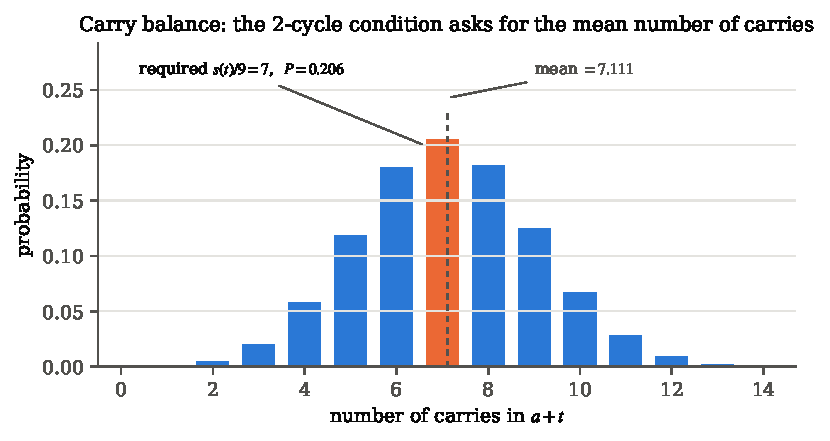
\includegraphics[width=0.92\textwidth]{figures/carry_balance.pdf}
\caption{Exact distribution of the number of carries in $a+t$ for a typical
$t=4536271809123471$ ($s(t)=63$), with $a$ random and odd. The $2$-cycle
condition requires $7=s(t)/9$ carries, next to the mean
$64/9\approx7.111$ (Theorem~\ref{thm:balance}); it holds with probability
$0.206$.}\label{fig:balance}
\end{figure}

This is the conceptual reason for everything in
Sections~\ref{sec:resonance}--\ref{sec:zero}: the carry count is a sum of
about $\log_{10}t$ weakly dependent terms, so it equals its mean with
probability of order $(\log t)^{-1/2}$ (Figure~\ref{fig:balance}), except when
the digits of $t$ are almost all $9$, where the count is nearly deterministic
and the probability is close to $9/10$. We now turn this into a sharp
theorem.

\begin{lemma}[Variance of carries]\label{lem:var}
Let $t\ge0$ and let $a_0,a_1,\dots,a_{k-1}$ be independent digits, where
$a_0$ may have any law and $\Pr(a_i=d)\ge\delta$ for all $d\in\{0,\dots,9\}$
and $1\le i\le k-1$. Let $c_j$ be the carry out of column $j-1$
($1\le j\le k$), so that $\C_k(a,t)=\sum_{j=1}^kc_j$. Then
\[
  |\operatorname{Cov}(c_i,c_j)|\le(1-9\delta)^{\,j-i}\quad(1\le i<j\le k),
  \qquad
  \operatorname{Var}\C_k(a,t)\le\Bigl(1+\frac2{9\delta}\Bigr)k .
\]
\end{lemma}

\begin{proof}
Fix $1\le i<j\le k$. The carry $c_j$ is a function of $c_i$ and of the digits
in columns $i,\dots,j-1$, all of which are at least $1$ and independent of
$c_i$. Run the carry recursion through these columns twice with the same
digits, once from carry-in $0$ and once from carry-in $1$. In column $l$ the
two runs produce the same carry-out unless $a_l+t_l=9$, an event of
probability $\Pr(a_l=9-t_l)\le1-9\delta$; once the runs agree they agree
forever. Hence, with $\Delta=\Pr(c_j=1\mid c_i=1)-\Pr(c_j=1\mid c_i=0)$,
$0\le\Delta\le(1-9\delta)^{j-i}$ by independence of the columns. Since
$\operatorname{Cov}(c_i,c_j)=\operatorname{Var}(c_i)\,\Delta$ and
$\operatorname{Var}(c_i)\le\frac14$, the covariance bound follows (with room
to spare). Note that $a_0$ is never used: column $0$ only influences
$c_1$, and the bound for pairs involving $c_1$ uses columns $1,\dots,j-1$.
Finally
\[
  \operatorname{Var}\C_k\le\sum_{j=1}^k\operatorname{Var}(c_j)
  +2\sum_{i<j}(1-9\delta)^{j-i}
  \le\frac k4+2k\sum_{d\ge1}(1-9\delta)^d\le\Bigl(1+\frac2{9\delta}\Bigr)k. \qedhere
\]
\end{proof}

\begin{lemma}[Local lower bound for switch sums]\label{lem:llt}
Let $\xi_1,\dots,\xi_n$ be independent Bernoulli variables with success
probabilities $p_i\in[\delta,1-\delta]$, and let $S=\sum_i\xi_i$,
$\mu=\sum_ip_i$, $V=\sum_ip_i(1-p_i)$. For every $A>0$ there are constants
$c_{A,\delta}>0$ and $n_{A,\delta}$, depending only on $A$ and $\delta$, such
that for all $n\ge n_{A,\delta}$, all such $p_1,\dots,p_n$ and every integer
$x$ with $|x-\mu|\le A\sqrt n$,
\[
  \Pr(S=x)\ge\frac{c_{A,\delta}}{\sqrt n}.
\]
\end{lemma}

\begin{proof}
Note $\delta(1-\delta)n\le V\le n/4$.

\emph{(a) Unimodality.} The generating polynomial
$\prod_i(1-p_i+p_iz)$ has only real roots, so its coefficients
$\Pr(S=j)$ form a log-concave, hence unimodal, sequence~\cite{Hoggar}.

\emph{(b) Normal approximation.} By the Berry--Esseen inequality for
independent, non-identically distributed summands~\cite{Petrov},
$\sup_y|\Pr(S\le y)-\Phi((y-\mu)/\sqrt V)|\le C_0\sum_i\mathbb E|\xi_i-p_i|^3/V^{3/2}
\le C_0/\sqrt V$, since $\mathbb E|\xi_i-p_i|^3\le p_i(1-p_i)$.

\emph{(c) Mass on each side.} Let $w=\lceil\sqrt V\,\rceil$,
$J_-=\{x-w,\dots,x-1\}$ and $J_+=\{x+1,\dots,x+w\}$. In standard units
$|x-\mu|/\sqrt V\le A':=A/\sqrt{\delta(1-\delta)}$, and each of $J_\pm$
corresponds to an interval of length at least $1-1/\sqrt V$ within distance
$A'+2$ of $0$. By (b), $\Pr(S\in J_\pm)\ge\eta-2C_0/\sqrt V$ with
$\eta=\tfrac12\varphi(A'+2)$, where $\varphi$ is the standard normal density;
this is at least $\eta/2$ once $n$ is large in terms of $A,\delta$.

\emph{(d) Point mass.} Let $M$ be a mode of $S$. If $M\ge x$, unimodality gives
$\Pr(S=y)\le\Pr(S=x)$ for all $y\in J_-$, so
$\eta/2\le\Pr(S\in J_-)\le w\Pr(S=x)$. If $M<x$, the same argument applies to
$J_+$. In both cases $\Pr(S=x)\ge\eta/(2w)\ge\eta/(4\sqrt V)\ge\eta/(2\sqrt n)$.
\end{proof}

\begin{theorem}[Exact order of the $2$-cycle density]\label{thm:sharp}
There are absolute constants $c,K>0$ and $D_0$ such that for all $D\ge D_0$
\[
  \frac{c}{\sqrt{\log D}}\;\le\;\frac{T(D)}{10^D}\;\le\;\frac{K}{\sqrt{\log D}} .
\]
Equivalently, the number of $2$-cycles with odd point below $N$ is of exact
order $N/\sqrt{\log\log N}$.
\end{theorem}

\paragraph{Plan of the lower bound.} The proof conditions in three nested
layers. Each layer fixes part of the randomness and keeps the rest
independent, and Table~\ref{tab:plan} lists the objects involved.
\begin{enumerate}
\item \emph{Digit counts.} Fixing the multiset $N$ of digits of $a$ fixes
$t=s(a)$ and the target $m=s(t)/9$. Given $N$, the arrangement of the digits
is uniform. By Lemma~\ref{lem:sampling}, its lowest $k=O(\log D)$ digits may
be replaced by \emph{independent} digits with law $p_d=N_d/D$, at a cost of
$k^2/(2D)$.
\item \emph{Non-switch digits.} Under the independent law we condition on $G$,
which consists of all digits except those at the active switches $W$. The set
$W$ is a function of $G$: whether $i\in S(t)$ is active depends only on
$a_{i+1}$, and $i+1$ is even, so it is never itself a switch. The remaining
digits $a_i$, $i\in W$, are independent of $G$ and of each other, and each
influences only the carry out of its own column. Therefore
$\C_k=C_0+\sum_{i\in W}\xi_i$ with $C_0$ determined by $G$ and independent
Bernoulli summands $\xi_i$.
\item \emph{Good conditionings.} Two events determined by $G$ make the local
estimate applicable. $B_1$ says that the conditional mean $C_0+\mu_W$ is within
$2R\sqrt k$ of $m$. It has probability at least $\frac12$ because the
unconditional carry count is concentrated near $m$ (carry balance and the
variance lemma) and the Bernoulli part is concentrated near its mean. $B_2$
says that $|W|$ is of order $h$; it fails with probability
$e^{-\Omega(h)}$ by the Chernoff bound. On $B_1\cap B_2$ the target
$x=m-C_0$ of the Bernoulli sum lies within $A\sqrt{|W|}$ of its mean, with
$A$ bounded because $k=O(h)$. Lemma~\ref{lem:llt} then gives probability of
order $1/\sqrt{|W|}\asymp1/\sqrt{\log D}$.
\end{enumerate}

\begin{table}[h]
\centering
\small
\begin{tabular}{>{\raggedright}p{2.3cm}>{\raggedright}p{3.6cm}>{\raggedright\arraybackslash}p{6.8cm}}
\toprule
object & determined by & role\\
\midrule
$N$, $t$, $m$ & digit multiset & fixes the target; arrangement uniform given $N$\\
$A'$, $U'$ & $N$ & typical counts; $t\equiv9$ (mod $18$) with $\ge h/5$ switch positions\\
$p$ & $N$ & independent-digit approximation of the low digits\\
$W\subseteq S(t)$ & digits at even positions (part of $G$) & active switches: $a_{i+1}+t_{i+1}\ne9$\\
$G$ & all digits outside $W$ (incl.\ $a_0$) & fixes $C_0$ and the thresholds $\theta_i$\\
$\xi_i$, $i\in W$ & $a_i$ & independent Bernoulli given $G$, parameters in $[\delta,1-\delta]$\\
$B_1$, $B_2$ & $G$ & conditional mean near $m$; many switches\\
$x=m-C_0$ & $G$ & target for $\sum\xi_i$, within the local-limit window\\
\bottomrule
\end{tabular}
\caption{The objects in the proof of the lower bound in
Theorem~\ref{thm:sharp}.}\label{tab:plan}
\end{table}

\begin{proof}
The upper bound is Theorem~\ref{thm:zero}. For the lower bound we keep the
notation of its proof: $\ell$ is the number of digits of $9D$,
$h=\lfloor\log_{10}(\sqrt D/\log D)\rfloor$, $r=\lceil4\log_{10}D\rceil$,
$k=\ell+r$ and $\delta=1/20$. For large $D$,
\begin{equation}\label{eq:hk}
  \tfrac14\log_{10}D\le h,\qquad k\le6\log_{10}D .
\end{equation}
All constants below depend only on $\delta$ and on absolute constants, never
on $D$.

\emph{Step 1: typical digit counts and digit sums.} Let $A'$ be the event
$\max_d|N_d/D-\tfrac1{10}|\le\log D/\sqrt D$; by Hoeffding's inequality
$\Pr(A'^c)=O(D^{-2})$. Let $U'$ be the event that $t\equiv9\pmod{18}$ and
$|S(t)\cap[1,h)|\ge h/5$. Both conditions depend only on $t\bmod9\cdot10^h$.
Under the uniform law on $\mathbb Z/9\cdot10^h\cong\mathbb Z/9\times\mathbb Z/10^h$,
the residue mod $9$ is uniform and independent of the last $h$ digits, so
$t\equiv0\pmod9$ has probability $1/9$; the units digit is odd with
probability $1/2$; and, independently of the units digit, at least $h/5$ of
the roughly $h/2$ odd positions below $h$ carry a digit in $\{1,\dots,8\}$
with probability at least $1-e^{-c_1h}$. By Lemma~\ref{lem:lowdigits} with
$M=9\cdot10^h$,
\[
  \Pr(U')\ge\tfrac1{18}\bigl(1-e^{-c_1h}\bigr)-K_2\,\frac{9\cdot10^h}{\sqrt D}
  \ge\tfrac1{20}\quad\text{for large }D.
\]

\emph{Step 2: reduction to independent digits.} Fix digit counts $N$ in $A'$
such that $t=t(N)$ satisfies $U'$, and let $m=s(t)/9$. Then $p_d=N_d/D\ge1/20$
for all $d$. Given $N$, $a$ is a uniform arrangement, and
$E\supseteq\{a_0\text{ odd},\ \C_k(a,t)=m\}\setminus F$, where $F$ is the
event that a carry passes column $k-1$; as in Theorem~\ref{thm:zero},
$\Pr(F\mid N)\le(3/5)^r$. By Lemma~\ref{lem:sampling},
\begin{equation}\label{eq:reduce}
  \Pr(E\mid N)\ge\Pr\nolimits_p\bigl(a_0\text{ odd},\ \C_k=m\bigr)-\frac{k^2}{2D}-(3/5)^r,
\end{equation}
where $\Pr_p$ refers to independent digits with law $p$. We bound the first
term from below by $\Pr_p(a_0\text{ odd})\cdot\Pr_p(\C_k=m\mid a_0\text{ odd})$
with $\Pr_p(a_0\text{ odd})\ge\tfrac12-5\log D/\sqrt D\ge\tfrac14$.

\emph{Step 3: the carry count is concentrated near $m$.} Let $X=\C_k$ under
$\Pr_p(\cdot\mid a_0\text{ odd})$. Under uniform digits with $a_0$ odd,
Theorem~\ref{thm:balance} gives $\mathbb EX=m+\bigl(1-(t+1)10^{-k}\bigr)/9$.
The laws of $(a_0,\dots,a_{k-1})$ under $p$ and under the uniform law (both
conditioned on $a_0$ odd) differ in total variation by at most
$10k\log D/\sqrt D$, and $0\le X\le k$, so the mean changes by at most
$10k^2\log D/\sqrt D=o(1)$. Hence $|\mathbb EX-m|\le1$ for large $D$. By
Lemma~\ref{lem:var}, which allows column $0$ to have an arbitrary law (here:
uniform on the odd digits) and requires $\Pr(a_i=d)\ge\delta$ only for
$1\le i\le k-1$, we have $\operatorname{Var}X\le K_3k$ with
$K_3=1+2/(9\delta)$. Put $R=\max(1,4\sqrt{K_3})$. Chebyshev's
inequality gives, for $k\ge4$,
\[
  \Pr\bigl(|X-m|>R\sqrt k\bigr)\le\Pr\bigl(|X-\mathbb EX|>R\sqrt k-1\bigr)
  \le\frac{K_3k}{(R\sqrt k/2)^2}\le\frac14 .
\]

\emph{Step 4: switches.} Condition on $G$, the digits outside the switch set
$W$ of Lemma~\ref{lem:switch} (with $a_0$ included in $G$). Then
$X=C_0+\sum_{i\in W}\xi_i$, where $C_0$ is a function of $G$ and, given $G$,
the $\xi_i$ are independent Bernoulli variables with success probabilities
$p_i\in[\delta,1-\delta]$. Write $\mu_W=\sum_{i\in W}p_i$ and
$Y=\sum_{i\in W}\xi_i-\mu_W$. Since $\operatorname{Var}(Y\mid G)\le|W|/4\le k/4$,
Chebyshev's inequality gives $\Pr(|Y|>R\sqrt k)\le1/(4R^2)\le1/4$. As
$C_0+\mu_W-m=(X-m)-Y$, the event
\[
  B_1=\bigl\{|C_0+\mu_W-m|\le2R\sqrt k\bigr\},
\]
which is determined by $G$, satisfies $\Pr(B_1)\ge1-\tfrac14-\tfrac14=\tfrac12$.
Let $B_2=\{|W|\ge w_0\}$ with $w_0=\tfrac92\delta\cdot\tfrac h5$; also determined
by $G$. Since $|S(t)|\ge h/5$, the Chernoff bound in Lemma~\ref{lem:switch}
gives $\Pr(B_2^c)\le e^{-9\delta h/40}$. Hence
\[
  \Pr(B_1\cap B_2)\ge\tfrac12-e^{-9\delta h/40}\ge\tfrac14\quad\text{for large }D.
\]

\emph{Step 5: local lower bound.} On $B_1\cap B_2$, the target value
$x=m-C_0$ satisfies $|x-\mu_W|\le2R\sqrt k\le A\sqrt{|W|}$, where
$A=2R\sqrt{k/w_0}$ is bounded by an absolute constant because of~\eqref{eq:hk}.
Since $|W|\ge w_0\to\infty$, Lemma~\ref{lem:llt}, applied conditionally on $G$,
gives
\[
  \Pr(X=m\mid G)=\Pr\Bigl(\sum_{i\in W}\xi_i=x\Bigm|G\Bigr)
  \ge\frac{c_{A,\delta}}{\sqrt{|W|}}\ge\frac{c_{A,\delta}}{\sqrt k}
\]
uniformly on $B_1\cap B_2$. Therefore
$\Pr_p(\C_k=m\mid a_0\text{ odd})\ge\tfrac14\,c_{A,\delta}/\sqrt k\ge c_4/\sqrt{\log D}$
by~\eqref{eq:hk}.

\emph{Step 6: conclusion.} Combining with~\eqref{eq:reduce} and Step~2, for
every admissible $N$,
$\Pr(E\mid N)\ge\tfrac14c_4/\sqrt{\log D}-k^2/(2D)-(3/5)^r\ge c_5/\sqrt{\log D}$
for large $D$. Averaging over $N$,
\[
  \frac{T(D)}{10^D}=\Pr(E)\ge\Pr(A'\cap U')\cdot\frac{c_5}{\sqrt{\log D}}
  \ge\Bigl(\tfrac1{20}-O(D^{-2})\Bigr)\frac{c_5}{\sqrt{\log D}}
  \ge\frac{c}{\sqrt{\log D}}. \qedhere
\]
\end{proof}

\begin{figure}[t]
\centering
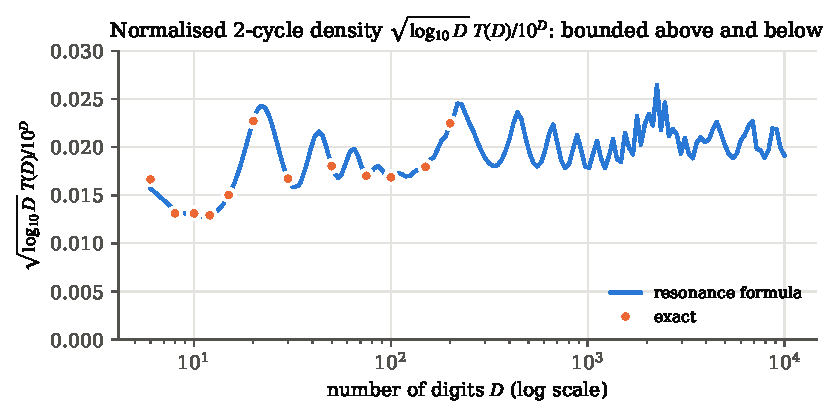
\includegraphics[width=0.92\textwidth]{figures/normalized_density.pdf}
\caption{The $2$-cycle density multiplied by $\sqrt{\ln D}$ stays between
positive bounds, as Theorem~\ref{thm:sharp} asserts; the log-periodic
modulation of Figure~\ref{fig:density} remains.}\label{fig:normalized}
\end{figure}

\subsection{The oscillation law}\label{sec:osclaw}

We now determine the normalised density exactly, up to a factor $1+o(1)$. This
proves that it oscillates, identifies its limit points and shows that the
limiting peak-to-trough ratio is $\sqrt{301}/11\approx1.577$, well above the
values near $1.4$ seen in Table~\ref{tab:osc}. Three new ingredients are needed: an
exact formula for the variance of the carry count, a sharp extremal bound for
the digit averages that this formula involves, and a local limit theorem with
the sharp constant.

Throughout this subsection $a$ has independent digits, $a_0$ uniform on
$\{1,3,5,7,9\}$ and $a_i$ uniform on $\{0,\dots,9\}$ for $i\ge1$. For $t\ge0$ let
$c_i$ ($i\ge1$) be the carry into column $i$ of $a+t$, let $q_i=\Pr(c_i=1)$,
and let $C=C(a,t)=\sum_{i\ge1}c_i$. Then $\rho(t)=\Pr(C=s(t)/9)$. Write
$\{y\}$ for the fractional part of a real number $y$ and
\[
  \varphi(x)=x(1-x).
\]

\begin{lemma}[Exact carry variance]\label{lem:exactvar}
For every $t\ge0$ and $1\le i\le j$,
\[
  q_{i+1}=\frac{t_i+q_i}{10},\qquad
  \operatorname{Cov}(c_i,c_j)=10^{-(j-i)}\,q_i(1-q_i),\qquad
  \operatorname{Var}C=\frac{11}9\sum_{i\ge1}\varphi(q_i).
\]
Moreover $|q_i-\{t/10^i\}|\le10^{1-i}$ for all $i\ge1$.
\end{lemma}

\begin{proof}
Given $c_i=c$, column $i$ carries out iff $a_i\ge10-t_i-c$, which has
probability $(t_i+c)/10$ (also when $t_i+c=10$). So
$\mathbb E[c_{i+1}\mid c_1,\dots,c_i]=(t_i+c_i)/10$. Taking expectations
gives the recursion for $q_i$. Subtracting it gives
$\mathbb E[c_{i+1}-q_{i+1}\mid c_1,\dots,c_i]=(c_i-q_i)/10$, and by induction
$\mathbb E[c_j-q_j\mid c_1,\dots,c_i]=10^{-(j-i)}(c_i-q_i)$. Multiplying by
$c_i-q_i$ and taking expectations gives the covariance. Above the top digit
of $t$ we have $t_i=0$ and $q_{i+1}=q_i/10$, so $\sum_iq_i<\infty$ and all
the series below converge absolutely. Hence
\[
  \operatorname{Var}C=\sum_i\varphi(q_i)\Bigl(1+2\sum_{d\ge1}10^{-d}\Bigr)
  =\frac{11}9\sum_i\varphi(q_i).
\]
Finally $x_i=\{t/10^i\}=(t\bmod10^i)/10^i$ satisfies $x_1=t_0/10$ and
$x_{i+1}=(t_i+x_i)/10$, so $q_i-x_i=10^{1-i}(q_1-x_1)$, and
$|q_1-x_1|\le1$.
\end{proof}

So the variance of the carry count is an additive functional of the
fractional parts $\{t/10^i\}$. A digit $9$ or $0$ in $t$ pushes the next
fractional part towards $1$ or $0$, where $\varphi$ vanishes. This is the
exact form of the resonance mechanism.

\begin{lemma}[Extremal digit averages]\label{lem:kappa}
Let $x_1\in[0,1]$, let $d_1,\dots,d_n\in\{0,\dots,9\}$ and
$x_{i+1}=(d_i+x_i)/10$. Then
\[
  \sum_{i=1}^n\varphi(x_i)\le\frac{30}{121}\,n+\frac5{22}.
\]
The constant $30/121$ is best possible: for the digits $4,5,4,5,\dots$ the
points $x_i$ converge to the $2$-cycle $\{5/11,6/11\}$, where
$\varphi=30/121$.
\end{lemma}

\begin{proof}
Put $u_i=x_i-\frac12\in[-\frac12,\frac12]$ and $e_i=d_i-\frac92$, so that
$u_{i+1}=(e_i+u_i)/10$ and $|e_i|\ge\frac12$. For $\alpha=\frac1{11}$,
$\beta=\frac1{110}$ and all real $u$ and $e$ with $|e|\ge\frac12$,
minimising over $u$ gives
\[
  \alpha u^2+\beta(u+e)^2\ \ge\ \frac{\alpha\beta}{\alpha+\beta}\,e^2
  =\frac{e^2}{121}\ \ge\ \frac1{484}.
\]
With $u=u_i$, $e=e_i$ and $\beta(u_i+e_i)^2=\frac{10}{11}u_{i+1}^2$ this reads
$u_i^2-\frac1{484}\ge\frac{10}{11}\bigl(u_i^2-u_{i+1}^2\bigr)$. Summing,
$\sum_{i=1}^nu_i^2\ge\frac n{484}-\frac{10}{11}\cdot\frac14$. Since
$\varphi(x_i)=\frac14-u_i^2$, the bound follows. The $2$-cycle: the composition
$x\mapsto(4+(5+x)/10)/10$ fixes $5/11$, and $(5+5/11)/10=6/11$.
\end{proof}

\begin{lemma}[Smoothness of Bernoulli sums]\label{lem:smooth}
Let $S$ be a sum of $n\ge1$ independent Bernoulli variables with success
probabilities in $[\delta,1-\delta]$. Then for every integer $x$
\[
  |\Pr(S=x+1)-\Pr(S=x)|\le\frac{\pi}{4\delta(1-\delta)\,n}.
\]
\end{lemma}

\begin{proof}
Let $\psi(\theta)=\mathbb Ee^{i\theta S}$. For each summand,
$|1-p+pe^{i\theta}|^2=1-2p(1-p)(1-\cos\theta)\le
\exp(-4\delta(1-\delta)\theta^2/\pi^2)$ for $|\theta|\le\pi$, using
$1-\cos\theta\ge2\theta^2/\pi^2$. So
$|\psi(\theta)|\le e^{-c n\theta^2}$ with $c=2\delta(1-\delta)/\pi^2$. By
Fourier inversion,
\[
  |\Pr(S=x+1)-\Pr(S=x)|=\Bigl|\frac1{2\pi}\int_{-\pi}^{\pi}
  e^{-ix\theta}(e^{-i\theta}-1)\psi(\theta)\,d\theta\Bigr|
  \le\frac1{2\pi}\int_{-\infty}^{\infty}|\theta|e^{-cn\theta^2}d\theta
  =\frac1{2\pi cn}. \qedhere
\]
\end{proof}

\begin{theorem}[Sharp local limit theorem for carries]\label{thm:sharpllt}
For every $\lambda\in(0,1]$ and $\varepsilon>0$ there is $n_0$ with the
following property. Let $t$ have $\ell$ digits and suppose its switch set
$S(t)$ (Lemma~\ref{lem:switch}) has $|S(t)|\ge\max(n_0,\lambda\ell)$. Then
$V=\operatorname{Var}C$ and $\mu=\mathbb EC$ satisfy, for every integer $m$ with
$|m-\mu|\le1$,
\[
  \Bigl|\sqrt{2\pi V}\,\Pr(C=m)-1\Bigr|\le\varepsilon .
\]
\end{theorem}

\begin{proof}
Let $p(x)=\Pr(C=x)$ and $\delta=\frac1{10}$.

\emph{Size of $V$.} Lemma~\ref{lem:switch} (whose proof applies to the full
carry count) gives $C=C_0+\sum_{i\in W}\xi_i$, where, given the digits $G$
outside $W$, the $\xi_i$ are independent Bernoulli variables with
parameters in $[\delta,1-\delta]$, and $\Pr(i\in W)\ge9\delta$ independently
over $i\in S(t)$. Hence $V\ge\mathbb E\operatorname{Var}(C\mid G)\ge
\delta(1-\delta)\,\mathbb E|W|\ge0.08\,|S(t)|$. In the other direction,
Lemma~\ref{lem:exactvar} gives $V\le\frac{11}9(\frac\ell4+\sum_{i>\ell}q_i)
\le\ell/3+1\le(1/\lambda+1)|S(t)|$, because $q_i\le10^{\ell-i}$ for $i>\ell$.

\emph{Smoothness.} Given $G$, $p(\cdot\mid G)$ is a shift of the law of a
Bernoulli sum with $|W|$ terms, so Lemma~\ref{lem:smooth} and the Chernoff
bound $\Pr(|W|<\frac92\delta|S(t)|)\le e^{-9\delta|S(t)|/8}$ give
\[
  \sup_x|p(x+1)-p(x)|\le L:=\frac{K}{|S(t)|}+e^{-|S(t)|/90}
\]
for an absolute constant $K$.

\emph{Central limit theorem.} (General local limit theorems for
non-homogeneous chains~\cite{DolgopyatSarig} assume uniform ellipticity,
which fails here when $t_i\in\{0,9\}$; we therefore combine a central limit
theorem with the smoothing above.) The carries $c_1,c_2,\dots$ form a
non-homogeneous Markov chain on $\{0,1\}$. Its $i$-th transition matrix has
rows $(1-\frac{t_i}{10},\frac{t_i}{10})$ and
$(1-\frac{t_i+1}{10},\frac{t_i+1}{10})$, so its Dobrushin contraction
coefficient $\delta_i=\frac12\sum_y|P_i(0,y)-P_i(1,y)|$ equals $\frac1{10}$, for
every $i$ and every $t$; the ergodic coefficient is $\alpha_i=1-\delta_i=\frac9{10}$.
We use Dobrushin's theorem in the form of Sethuraman and
Varadhan~\cite[Thm.~1.1]{SethuramanVaradhan}. For a triangular array of
non-homogeneous Markov chains $X^{(n)}_1,\dots,X^{(n)}_{k_n}$ and functions
$f^{(n)}_i$ with $|f^{(n)}_i|\le C_n$, let $\alpha_n$ be the smallest ergodic
coefficient in row $n$ and $S_n=\sum_if^{(n)}_i(X^{(n)}_i)$. If
$C_n^2\alpha_n^{-3}/\sum_i\operatorname{Var}f^{(n)}_i(X^{(n)}_i)\to0$, then
$(S_n-\mathbb ES_n)/\sqrt{\operatorname{Var}S_n}$ converges in law to the
standard normal. In our case $f_i(c)=c$, $C_n=1$ and $\alpha_n=\frac9{10}$, and
$\sum_i\operatorname{Var}c_i=\sum_i\varphi(q_i)=\frac9{11}V$ by
Lemma~\ref{lem:exactvar}. So the condition is simply $V\to\infty$.

To make this uniform in $t$, suppose it fails. Then there are
$\varepsilon'>0$ and digit strings $t^{(n)}$ with $V(t^{(n)})\to\infty$ such that
$\sup_y|\Pr(C\le\mu+y\sqrt V)-\Phi(y)|>\varepsilon'$ for every $n$. Truncate
the $n$-th chain after column $k_n=\ell_n+r_n$ with $r_n\to\infty$. This
changes $C$ with probability at most $\sum_{i>k_n}q_i\le10^{-r_n}$, and
changes $V$ by a factor $1+o(1)$. The array of truncated chains satisfies the
condition above, so $(C-\mu)/\sqrt V$ converges in law to $N(0,1)$ along
$t^{(n)}$. By P\'olya's theorem the convergence is uniform in $y$, because
$\Phi$ is continuous. This contradicts the choice of $t^{(n)}$. Hence for every
$\varepsilon'>0$ there is $V_0$ with
$\sup_y|\Pr(C\le\mu+y\sqrt V)-\Phi(y)|\le\varepsilon'$ whenever
$V(t)\ge V_0$.

\emph{Combination.} Fix $\eta\in(0,1)$ and let
$J=\{x\in\mathbb Z:|x-m|\le\eta\sqrt V\}$, so $\bigl||J|-2\eta\sqrt V\bigr|\le1$.
For $x\in J$, $|p(x)-p(m)|\le L\eta\sqrt V$, so
$\bigl|\sum_{x\in J}p(x)-|J|\,p(m)\bigr|\le|J|\,L\eta\sqrt V$. Since
$|m-\mu|\le1$, the central limit theorem gives
$\sum_{x\in J}p(x)=2\eta\,\phi(0)\bigl(1+O(\eta^2+V^{-1/2})\bigr)+O(\varepsilon')$,
with $\phi(0)=1/\sqrt{2\pi}$. Dividing by $|J|$,
\[
  \sqrt V\,p(m)=\phi(0)\bigl(1+O(\eta^2+V^{-1/2})\bigr)
  +O\Bigl(\frac{\varepsilon'}\eta+\frac1{\eta\sqrt V}\Bigr)+O(L\eta V).
\]
By the bounds on $V$, $L\eta V\le K'\eta/\lambda$ once $|S(t)|$ is large. Choose
$\eta$ so small that the $\eta$-terms are below $\varepsilon/3$, then
$\varepsilon'=\varepsilon\eta/3$, and then $n_0$ so large that
$V\ge0.08n_0\ge V_0$ and the remaining terms are below $\varepsilon/3$.
\end{proof}

\begin{theorem}[Oscillation law]\label{thm:osclaw}
Let $h=h_D=\lfloor\log_{10}(\sqrt D/\log D)\rfloor$ and
\[
  B_D=\sum_{i>h}\varphi\bigl(\{4.5D/10^i\}\bigr).
\]
Then, as $D\to\infty$,
\[
  \frac{T(D)}{10^D}=\frac{1+o(1)}{36\sqrt{\frac{22\pi}9\bigl(\frac h6+B_D\bigr)}} .
\]
\end{theorem}

\paragraph{Error budget.} The main term is of order $(\log D)^{-1/2}$.
Table~\ref{tab:budget} lists the five sources of error in the proof, each of
which is smaller than the main term.

\begin{table}[h]
\centering
\small
\begin{tabular}{>{\raggedright}p{3.1cm}>{\raggedright}p{5.6cm}>{\raggedright\arraybackslash}p{4cm}}
\toprule
component & what is shown & error\\
\midrule
resonance approximation & $T(D)/10^D=\frac12\sum_tP_D(t)\rho(t)+\text{error}$ (Theorem~\ref{thm:resrig}) & $O((\log D)^2/\sqrt D)$\\
bad digit sums & (G1) fails, or (G2) fails, or (G3) fails & $e^{-c\log^2D}+O(1/\log D)+O((\log D)^{-3/4})$\\
variance of good $t$ & $V(t)=\frac{11}9(\frac h6+B_D)(1+o(1))$ & relative $O(\varepsilon_D+\log\log D/\log D)$\\
local limit & $\rho(t)=(1+o(1))(2\pi V(t))^{-1/2}$ (Theorem~\ref{thm:sharpllt}) & relative $o(1)$, uniform in good $t$\\
mass of good $t$ & $\frac12P_D(\text{good})=\frac1{36}+o(1)$ (Lemma~\ref{lem:lowdigits}) & $O(1/\log D)$\\
\bottomrule
\end{tabular}
\caption{Error budget for Theorem~\ref{thm:osclaw}, with
$\varepsilon_D=(\log D)^{-1/8}$. Absolute errors are $o((\log D)^{-1/2})$;
relative errors multiply the main term by $1+o(1)$.}\label{tab:budget}
\end{table}

\begin{proof}
By Theorem~\ref{thm:resrig} it suffices to evaluate
$\frac12\sum_{t\equiv9\,(18)}P_D(t)\rho(t)$ up to a factor $1+o(1)$; the error
there is $O((\log D)^2/\sqrt D)$, while the claimed main term is of order
$(\log D)^{-1/2}$. Let $\varepsilon_D=(\log D)^{-1/8}$ and
$x_i(y)=\{y/10^i\}$. Call $t\equiv9\pmod{18}$ \emph{good} if
\begin{enumerate}
\item[(G1)] $|t-4.5D|\le\sqrt D\log D$;
\item[(G2)] $|S(t)\cap[1,h)|\ge h/5$;
\item[(G3)] $\bigl|\sum_{i=1}^h\varphi(x_i(t))-h/6\bigr|\le\varepsilon_Dh$.
\end{enumerate}
\emph{Bad $t$ are negligible.} (G1) fails with probability
$e^{-c\log^2D}$. Conditions (G2), (G3) and $t\equiv9\pmod{18}$ depend only
on $t\bmod9\cdot10^h$, whose law is within total variation
$9K_2\,10^h/\sqrt D\le9K_2/\log D$ of uniform (Lemma~\ref{lem:lowdigits}).
Under the uniform law, $t\equiv0\pmod9$ and $t$ odd have probability
$\frac1{18}$ jointly, and independently of them the digits $t_1,\dots,t_{h-1}$
are uniform and independent. Then (G2) fails with probability $e^{-ch}$, as
in Theorem~\ref{thm:zero}. For (G3), each $x_i$ is uniform on the grid
$10^{-i}\mathbb Z\cap[0,1)$, so $\mathbb E\varphi(x_i)=\frac16-\frac1{6}10^{-2i}$.
Also $\varphi(x_j)$ differs by at most $10^{-(j-i)}$ from a function of
$t_{i},\dots,t_{j-1}$, which is independent of $x_i$; so
$|\operatorname{Cov}(\varphi(x_i),\varphi(x_j))|\le2\cdot10^{-(j-i)}$ and the
variance of the sum is $O(h)$. By Chebyshev's inequality (G3) fails with
probability $O(1/(\varepsilon_D^2h))=O((\log D)^{-3/4})$. Since $\rho\le1$, bad
$t$ contribute $o((\log D)^{-1/2})$.

\emph{Variance of good $t$.} By Lemma~\ref{lem:exactvar}, and since $\varphi$
is $1$-Lipschitz, $V(t)=\frac{11}9\bigl(\sum_{i\ge1}\varphi(x_i(t))+O(1)\bigr)$.
The terms $i\le h$ contribute $h/6+O(\varepsilon_Dh)$ by (G3). Let
$\omega=\lceil3\log_{10}\log D\rceil+2$. The terms $h<i\le h+\omega$ of both
$\sum_i\varphi(x_i(t))$ and $B_D$ are at most $\omega/4$ in total. For $i>h+\omega$,
$\varphi$ is $1$-Lipschitz on $\mathbb R/\mathbb Z$ (since $\varphi(0)=\varphi(1)$), so
$|\varphi(x_i(t))-\varphi(x_i(4.5D))|\le|t-4.5D|/10^i$. By (G1) and
$10^h\ge\sqrt D/(10\log D)$, these differences sum to at most
$20\log^2D/10^{\omega}\le1$. Hence
\[
  V(t)=\frac{11}9\Bigl(\frac h6+B_D\Bigr)\bigl(1+o(1)\bigr)
\]
uniformly over good $t$, because $h/6+B_D\ge h/6$ and the errors are
$O(\varepsilon_Dh+\log\log D)=o(h)$.

\emph{Local limit.} A good $t$ has $\ell\le\log_{10}D+2\le3h$ digits for large
$D$ and $|S(t)|\ge h/5\ge\ell/15$. By Theorem~\ref{thm:balance} (letting
$K\to\infty$) $\mu=\mathbb EC=(s(t)+1)/9$, so the target $m=s(t)/9$ satisfies
$|m-\mu|=\frac19$. Theorem~\ref{thm:sharpllt} with $\lambda=\frac1{15}$ gives
$\rho(t)=(1+o(1))(2\pi V(t))^{-1/2}$ uniformly over good $t$.

\emph{Conclusion.} The good $t$ carry
$\frac12P_D(\text{good})=\frac1{36}+o(1)$, and on them
$\rho(t)=(1+o(1))\bigl(\frac{22\pi}9(\frac h6+B_D)\bigr)^{-1/2}$.
\end{proof}

\begin{corollary}[The normalised density oscillates]\label{cor:osc}
Let $\Phi(D)=\sqrt{\log_{10}D}\;T(D)/10^D$ and $K_0=1/(12\sqrt{11\pi})$. Then
\[
  \limsup_{D\to\infty}\Phi(D)=K_0\sqrt6\approx0.03472,\qquad
  \liminf_{D\to\infty}\Phi(D)=K_0\sqrt{\tfrac{726}{301}}\approx0.02201,
\]
and the set of limit points of $\Phi(D)$ is the whole interval between them.
Moreover $\Phi(D)\to K_0\sqrt3\approx0.02455$ for almost all $D$: for every
$\varepsilon>0$, the proportion of $D\in[10^j,10^{j+1})$ with
$|\Phi(D)-K_0\sqrt3|>\varepsilon$ tends to $0$ as $j\to\infty$.
In particular $\Phi(D)$ has no limit, and
\[
  \frac{\limsup\Phi}{\liminf\Phi}=\frac{\sqrt{301}}{11}=1.5772\ldots
\]
The $\limsup$ is approached along $D=\lfloor10^j/4.5\rfloor$, where the top
digits of the typical digit sum are nines. The $\liminf$ is approached along
$D=\lfloor\frac29\,y_j\rfloor$, where $y_j=4545\cdots$ has $j$ digits. The same
holds with $\sqrt{\ln D}$ in place of $\sqrt{\log_{10}D}$, all values multiplied
by $\sqrt{\ln10}$.
\end{corollary}

\begin{proof}
Let $\ell_D$ be the number of digits of $\lfloor4.5D\rfloor$. Then
$h/\log_{10}D\to\frac12$ and $(\ell_D-h)/\log_{10}D\to\frac12$. Positions
$i>\ell_D$ contribute at most $\sum_{i>\ell_D}10^{\ell_D-i}\le\frac19$ to $B_D$,
so Lemma~\ref{lem:kappa} gives
$0\le B_D\le\frac{30}{121}(\ell_D-h)+1$. Write
$B_D=\frac12\log_{10}D\cdot\beta_D$. Then
$0\le\beta_D\le\frac{30}{121}+o(1)$, and Theorem~\ref{thm:osclaw} becomes
\[
  \Phi(D)=\frac{1+o(1)}{36\sqrt{11\pi/9}}\Bigl(\frac16+\beta_D\Bigr)^{-1/2}
  =K_0\Bigl(\frac16+\beta_D\Bigr)^{-1/2}+o(1),
\]
with $\frac16+\frac{30}{121}=\frac{301}{726}$. For $D=\lfloor10^j/4.5\rfloor$
we have $10^j-4.5<4.5D\le10^j$. So $\varphi(\{4.5D/10^i\})\le4.5\cdot10^{-i}$ for
$i\le j$ and $\le10^{j-i}$ for $i>j$, giving $B_D=O(1)$ and $\beta_D\to0$. For
$D=\lfloor\frac29y_j\rfloor$, $\{4.5D/10^i\}$ lies within $6\cdot10^{-i}$ of
$5/11$ or $6/11$ for $h<i\le j$. So $B_D\ge\frac{30}{121}(j-h)-O(1)$ and
$\beta_D\to\frac{30}{121}$. Finally, $|B_{D+1}-B_D|\le\sum_{i>h}4.5\cdot10^{-i}
\to0$ because $\varphi$ is $1$-Lipschitz on the circle. Hence
$\Phi(D+1)-\Phi(D)\to0$, and a sequence with vanishing increments that
oscillates between two values has every intermediate value as a limit point.

For the typical value, let $D$ be uniform in $[10^j,10^{j+1})$ and
$\omega=\lceil\log_{10}j\rceil$. Writing $D=2u$ or $2u+1$ gives
$\lfloor4.5D\rfloor=9u$ or $9u+4$, and $u$ runs over more than $10^j/2$
consecutive integers. Since $\gcd(9,10)=1$, the residue of $\lfloor4.5D\rfloor$
modulo $10^{j-\omega}$ is within total variation $O(10^{-\omega})$ of uniform.
So its digits in positions $h,\dots,j-\omega$ are close to independent and
uniform, and, as in step (G3) of the proof of Theorem~\ref{thm:osclaw}, the sum of
$\varphi(\{4.5D/10^i\})$ over these positions is $(j-h)/6+O_P(\sqrt j)$. The
top $\omega$ positions contribute $O(\omega)=o(j)$. So
$\beta_D\to\frac16$ in probability and
$\Phi(D)\to K_0(\frac16+\frac16)^{-1/2}=K_0\sqrt3$.
\end{proof}

\begin{figure}[t]
\centering
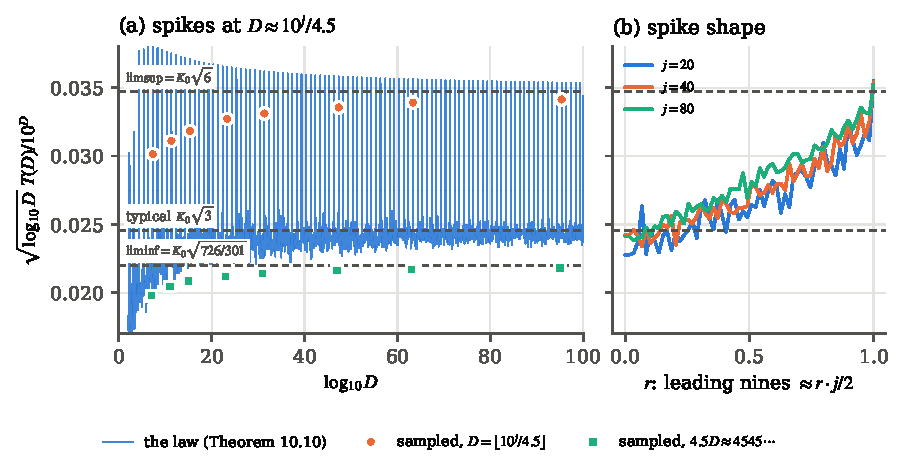
\includegraphics[width=\textwidth]{figures/oscillation_law.pdf}
\caption{The oscillation law. (a)~The main term of Theorem~\ref{thm:osclaw},
evaluated densely near the resonances $D\approx10^j/4.5$ and on a uniform grid
in $\log_{10}D$. For most $D$ it is close to the typical value $K_0\sqrt3$. Near
$D=10^j/4.5$ it spikes towards $K_0\sqrt6$, and near $4.5D\approx4545\cdots$ it
dips towards $K_0\sqrt{726/301}$. The finite-$D$ formula overshoots
$K_0\sqrt6$ for moderate $D$ because $h/\log_{10}D\to\frac12$ only
logarithmically. Circles and squares are sampled values of the exact main
term, $\frac12\sum_tP_D(t)\rho(t)$, at peaks and troughs, which approach the
proved limits. (b)~Spike shape: the law at
$D=(10^j/4.5)(1-10^{-rj/2})$, when the typical digit sum begins with about
$rj/2$ nines, for $j=20,40,80$. The curves rise from the typical value to the
peak in the same way for every $j$.}\label{fig:osclaw}
\end{figure}

\begin{remark}[Why Table~\ref{tab:osc} shows $1.4$]\label{rem:slow}
The approach to the limit is logarithmically slow. At $D\approx2\cdot10^7$ the
random part of the digit sum has only about four digits and the
deterministic part about four. The $O(1)$ boundary terms in $V(t)$ are then
comparable with the main terms. Evaluating the main term by sampling
$3000$ digit sums from the Gaussian window, with exact integer arithmetic, at
the peak $D=\lfloor10^j/4.5\rfloor$ and at the trough
$D=\lfloor\frac29y_j\rfloor$ gives ratios $1.524\pm0.005$, $1.519\pm0.003$,
$1.526\pm0.003$, $1.542\pm0.002$, $1.545\pm0.002$, $1.551\pm0.001$,
$1.562\pm0.001$ and $1.565\pm0.001$ for $j=8,12,16,24,32,48,64,96$. The
errors are one standard error, from the sample variances by the delta
method. The ratios increase towards $\sqrt{301}/11=1.5772$. The quantity
$\rho(t)\sqrt{2\pi V(t)}$ of Theorem~\ref{thm:sharpllt} averages $0.9865$,
$0.9948$, $0.9982$ and $0.9994$ over random $t$ with $10$, $30$, $100$ and
$300$ digits.
\end{remark}

\section{Other bases}\label{sec:bases}

For an integer base $b\ge2$ let $s_b(n)$ be the base-$b$ digit sum and
\[
  f_b(n)=\begin{cases}n+s_b(n),&n\text{ odd},\\ n-s_b(n),&n\text{ even}.\end{cases}
\]
Write $\C_b(x,y)$ and $\B_b(x,y)$ for the numbers of carries and borrows in
base $b$. The proof of Lemma~\ref{lem:carry} gives
$s_b(x+y)=s_b(x)+s_b(y)-(b-1)\C_b(x,y)$ and
$s_b(x-y)=s_b(x)-s_b(y)+(b-1)\B_b(x,y)$, and $s_b(n)\equiv n\pmod{b-1}$.
The behaviour of $f_b$ depends sharply on the parity of $b$.

\begin{theorem}[Odd bases]\label{thm:oddbase}
If $b$ is odd, every orbit of $f_b$ reaches the fixed point $0$; in particular
$f_b$ has no cycle other than $\{0\}$.
\end{theorem}

\begin{proof}
For odd $b$, $b\equiv1\pmod2$ gives $n\equiv s_b(n)\pmod2$. If $n$ is odd,
then $s_b(n)$ is odd and $f_b(n)=n+s_b(n)$ is even. If $n>0$ is even, then
$s_b(n)$ is even and positive, so $f_b(n)=n-s_b(n)$ is even, non-negative and
strictly smaller than $n$. Hence after at most one step the orbit consists of
even numbers that decrease strictly until they reach $0$.
\end{proof}

In an odd base, branching on the parity of $n$ is the same as branching on
the parity of $s_b(n)$, so $f_b$ coincides with the base-$b$ analogue of the
iteration in OEIS A243260~\cite{OEIS-A243260}. The two rules differ only in
even bases, and that is where all the structure lies.

\begin{theorem}[Even bases: structure]\label{thm:evenbase}
Let $b\ge2$ be even. Then, with $9$ replaced by $b-1$ and $10$ by $b$
throughout:
\begin{enumerate}
\item the parity of $n$ is the parity of its last digit; for $b\ge4$ every term
  after the first even term of an orbit is a multiple of $b-1$;
\item $s_b((b-1)m)=(b-1)\,\B_b(bm,m)$, and on multiples of $b-1$ the map is
  conjugate to $m\mapsto m\pm\kappa_b(m)$ with $\kappa_b(m)=s_b((b-1)m)/(b-1)$;
\item the level equation of Theorem~\ref{thm:level} holds with
  $\kappa_b(k)$;
\item if $s_b(x)$ is even and $s_b(f_b(x)+b-1)=s_b(x)$, then
  $f_b(f_b(x)+b-1)=x+b-1$;
\item an odd $a$ lies on a $2$-cycle if and only if $s_b(a)$ is odd and
  $s_b(s_b(a))=(b-1)\,\C_b(a,s_b(a))$;
\item for $a$ uniform on $\{0,\dots,b^K-1\}$,
  $\mathbb E\,\C_{b,K}(a,t)=\bigl(s_b(t)-t\,b^{-K}\bigr)/(b-1)$, and for $a$
  uniform on the odd numbers there and odd $t<b^K$,
  $\mathbb E\,\C_{b,K}(a,t)=\bigl(s_b(t)+1-(t+1)b^{-K}\bigr)/(b-1)$;
\item prefix lifting (Theorem~\ref{thm:lift}) and its error bound
  (Corollary~\ref{cor:lifterr}) hold with $10^L$ replaced by $b^L$ and $9D$ by
  $(b-1)D$.
\end{enumerate}
\end{theorem}

\begin{proof}
The proofs for $b=10$ use only the carry and borrow identities, the
congruence $s_b(n)\equiv n\pmod{b-1}$, and two consequences of the evenness of
$b$: the parity of $n$ is that of its last digit, and $b-1$ is odd, so that
adding $b-1$ swaps parity (used in (iv)). They therefore apply verbatim. In
(vi), the odd digits $1,3,\dots,b-1$ average $b/2$ and the even digits
$0,2,\dots,b-2$ average $b/2-1$, so $\mathbb Es_b(a)-\mathbb Es_b(a+t\bmod b^K)=1$,
and exactly $(t+1)/2$ odd $a$ overflow. All seven statements were also checked
by computer for $b\in\{2,4,6,8,10,16\}$.
\end{proof}

\begin{proposition}[Resonance in base $b$]\label{prop:resb}
For even $b$ and $j\ge1$, the probability that adding $t=b^j-1$ to a random
odd integer produces exactly $s_b(t)/(b-1)=j$ carries is $(b-1)/b$.
\end{proposition}

\begin{proof}
The units column gives $a_0+(b-1)\ge b$ because $a_0$ is odd, and each of the
next $j-1$ columns gives $a_i+(b-1)+1\ge b$; so all $j$ columns carry, and the
count is exactly $j$ iff column $j$ does not carry, i.e.\ $a_j\neq b-1$.
\end{proof}

For $b\ge4$ the switch lemma (Lemma~\ref{lem:switch}) applies with the
switch digits $t_i\in\{1,\dots,b-2\}$. In base $2$ there are no such digits,
and the switch mechanism takes a different form.

\begin{lemma}[Binary switch lemma]\label{lem:binswitch}
Let $t\ge1$ have $\ell$ binary digits, let $0<\delta\le\frac12$, and let
$a$ have independent bits with $\Pr(a_i=1)\in[\delta,1-\delta]$ for
$1\le i\le\ell$. Let
\[
  S_2(t)=\{\,i\equiv2\ (\mathrm{mod}\ 4),\ 2\le i\le\ell-2:\ t_{i-1}\ne t_i\,\}.
\]
Then for every integer $m$, the number $C$ of carries in $a+t$ (possibly
truncated after any fixed column $k>\ell$) satisfies
$\Pr(C=m)\le K_1\delta^{-2}|S_2(t)|^{-1/2}+e^{-\delta^2|S_2(t)|/8}$.
\end{lemma}

\begin{proof}
For $i\in S_2(t)$ call $i$ a \emph{switch} if $a_{i-1}=t_{i-1}$ and
$a_{i+1}=t_{i+1}$. The column triples $\{i-1,i,i+1\}$ for distinct
$i\in S_2(t)$ are disjoint, so these events are independent, each of
probability at least $\delta^2$. Let $W$ be the set of switches and condition
on $G$, the bits outside $\{a_i:i\in W\}$; $W$ is determined by $G$.

Let $i\in W$. In column $i-1$, $a_{i-1}+t_{i-1}=2t_{i-1}\in\{0,2\}$, so the
carry into column $i$ is $c_i=t_{i-1}=1-t_i$ whatever the carry into column
$i-1$ (a \emph{reset}). In column $i$, $a_i+t_i+c_i=a_i+1$, so the carry out
of column $i$ is $\xi_i=a_i$. In column $i+1$, $a_{i+1}+t_{i+1}\in\{0,2\}$, so
the carry out of column $i+1$ is $t_{i+1}$ whatever $\xi_i$ is (a
\emph{block}). Hence $a_i$ influences only the carry $\xi_i$, and as in
Lemma~\ref{lem:switch}, $C=C_0+\sum_{i\in W}\xi_i$ with $C_0$ a function of $G$
and the $\xi_i$ independent Bernoulli variables with parameters in
$[\delta,1-\delta]$. The Kolmogorov--Rogozin inequality and the Chernoff bound
for $|W|$ finish the proof exactly as in Lemma~\ref{lem:switch}.
\end{proof}

Thus binary switches sit at the places where the bits of $t$ change, and
resonance in base $2$ occurs when $t=2^j-1$ has no bit changes at all.

\begin{theorem}[Two-cycle density in every even base]\label{thm:evenb}
For every even $b\ge2$ there are constants $c_b,K_b>0$ and $D_b$ such that for
$D\ge D_b$
\[
  \frac{c_b}{\sqrt{\log D}}\;\le\;\frac{T_b(D)}{b^D}\;\le\;\frac{K_b}{\sqrt{\log D}},
\]
where $T_b(D)$ is the number of odd $a<b^D$ on a $2$-cycle of $f_b$.
\end{theorem}

\begin{proof}
We go through the proofs of Theorems~\ref{thm:zero} and~\ref{thm:sharp}
and record each change. Fix an even $b$. Let $a$ be uniform on
$\{0,\dots,b^D-1\}$, with digit counts $N=(N_0,\dots,N_{b-1})$ and $t=s_b(a)$,
and let $E$ be the event that $a$ is the odd point of a $2$-cycle. Let $\ell$
be the number of base-$b$ digits of $(b-1)D$, so $t<b^\ell$, and set
\[
  h=\Bigl\lfloor\log_b\frac{\sqrt D}{\log D}\Bigr\rfloor,\qquad
  r=\Bigl\lceil\frac{\log D}{\log(4/3)}\Bigr\rceil,\qquad k=\ell+r .
\]
Then $h\ge\frac14\log_bD$ and $k\le C_b\log D\le C_b'h$ for large $D$. All
constants below depend only on $b$.

\emph{(a) Characterisation.} By Theorem~\ref{thm:evenbase}(v),
\[
  E=\{a\text{ odd},\ t\text{ odd},\ \C_b(a,t)=m(t)\},\qquad m(t)=\frac{s_b(t)}{b-1},
\]
which is empty unless $(b-1)\mid s_b(t)$, i.e.\ $(b-1)\mid t$, since
$s_b(t)\equiv t\pmod{b-1}$. In particular $E\subseteq\{\C_b(a,t)=m(t)\}$.
Because $b$ is even, the parity of $a$ and of $t$ is that of their last digit.

\emph{(b) Typical digit counts.} Let $A'$ be the event
$\max_d|N_d/D-1/b|\le\log D/\sqrt D$. By Hoeffding's inequality
$\Pr(A'^c)=O_b(D^{-2})$. On $A'$, every $p_d=N_d/D$ lies in
$[\frac1{2b},\frac{3}{4}]$ for large $D$, so we take $\delta=1/(2b)$.

\emph{(c) Overflow beyond column $k-1$.} The digits of $t$ in columns
$\ell,\dots,k-1$ are $0$, so a carry passes column $k-1$ only if
$a_\ell=\dots=a_{k-1}=b-1$. Given $N\in A'$ this has probability at most
$(p_{b-1}+k/D)^r\le(3/4)^r\le D^{-1}$.

\emph{(d) Low digits of $t$.} The law of $t$ is the $D$-fold convolution of the
uniform law on $\{0,\dots,b-1\}$. It is log-concave, and by~\eqref{eq:KR} its
largest atom is $O_b(D^{-1/2})$. The proof of Lemma~\ref{lem:lowdigits} then
shows that $t\bmod M$ is within total variation $K_bM/\sqrt D$ of uniform. We
use $M=b^h$ and $M=(b-1)b^h$; since $\gcd(b-1,b^h)=1$, under the uniform law
on $\mathbb Z/(b-1)b^h$ the residue mod $b-1$ and the last $h$ digits are
independent and uniform.

\emph{(e) Switch sets.} For $b\ge4$ let $S(t)$ be the set of odd $i<h$ with
$t_i\in\{1,\dots,b-2\}$. The proof of Lemma~\ref{lem:switch} goes through
word for word with $9$ replaced by $b-1$. A switch is $i\in S(t)$ with
$a_{i+1}+t_{i+1}\neq b-1$, which has probability at least $(b-1)\delta$, and
the threshold $\theta_i=b-t_i-c_i$ lies in $\{1,\dots,b-1\}$. Under the
uniform law on the last $h$ digits, each odd position carries a digit in
$\{1,\dots,b-2\}$ with probability $(b-2)/b\ge\frac12$, so
$|S(t)|\ge h/5$ except with probability $e^{-c_bh}$. For $b=2$ we use
$S_2(t)$ and Lemma~\ref{lem:binswitch}. The bits $t_{i-1},t_i$ for distinct
$i\equiv2\pmod4$ are disjoint pairs of uniform bits, each pair unequal with
probability $\frac12$, so $|S_2(t)|\ge h/16$ except with probability
$e^{-ch}$. In both cases the conditional decomposition
\begin{equation}\label{eq:bdecomp}
  \C_{b,k}(a,t)=C_0+\sum_{i\in W}\xi_i ,
\end{equation}
holds, with $C_0$ a function of the digits $G$ outside $W$ and, given $G$,
independent Bernoulli $\xi_i$ with parameters in $[\delta,1-\delta]$. For
$b=2$, $\xi_i=a_i$. Moreover $|W|\ge c_b'h$ except with probability
$e^{-c_b''h}$, by the Chernoff bound.

\emph{(f) Upper bound.} Conditionally on $N\in A'$ with $|S(t)|$ (or
$|S_2(t)|$) at least $h/16$, Lemma~\ref{lem:sampling} (with $b$ digit values;
its proof does not use the number of values) replaces the first $k$ digits
by independent digits with law $p$ at cost $k^2/(2D)$. The
Kolmogorov--Rogozin inequality applied to~\eqref{eq:bdecomp} then gives
$\Pr(\C_{b,k}=m)\le K_b/\sqrt h$. Together with (b)--(d),
\[
  \frac{T_b(D)}{b^D}\le O(D^{-2})+e^{-c_bh}+\frac{K_bb^h}{\sqrt D}
  +\frac{K_b}{\sqrt h}+\frac{k^2}{2D}+D^{-1}=O_b\bigl((\log D)^{-1/2}\bigr).
\]

\emph{(g) Lower bound.} Let $U'$ be the event that $t$ is odd,
$t\equiv0\pmod{b-1}$ and the switch set below $h$ has at least $h/16$
elements. All three conditions depend only on $t\bmod(b-1)b^h$. By (d) and
(e), $\Pr(U')\ge\frac1{2(b-1)}(1-e^{-c_bh})-K_b(b-1)b^h/\sqrt D
\ge\frac1{4(b-1)}$ for large $D$. Fix $N\in A'$ with $t(N)\in U'$ and put
$m=s_b(t)/(b-1)$, which is an integer. As in Step 2 of
Theorem~\ref{thm:sharp},
\[
  \Pr(E\mid N)\ge\Pr\nolimits_p(a_0\text{ odd})\,
  \Pr\nolimits_p\bigl(\C_{b,k}=m\mid a_0\text{ odd}\bigr)-\frac{k^2}{2D}-D^{-1},
\]
and $\Pr_p(a_0\text{ odd})\ge\frac14$.

\emph{Mean.} Let $X=\C_{b,k}$ under $\Pr_p(\cdot\mid a_0\text{ odd})$. By
Theorem~\ref{thm:evenbase}(vi), under uniform digits
$\mathbb EX=m+\bigl(1-(t+1)b^{-k}\bigr)/(b-1)\in[m,m+1]$. The change from
uniform digits to law $p$ moves the mean by at most
$bk^2\log D/\sqrt D=o(1)$, so $|\mathbb EX-m|\le2$.

\emph{Variance.} In the proof of Lemma~\ref{lem:var}, two runs of the carry
recursion through column $l$ disagree only if $a_l+t_l=b-1$, which has
probability at most $1-(b-1)\delta$. The lemma therefore holds in base $b$ with
$\operatorname{Var}X\le K_3k$ and $K_3=1+2/((b-1)\delta)$. Column $0$ again has an
arbitrary law.

\emph{Concentration and switches.} Put $R=\max(2,4\sqrt{K_3})$. Since
$|\mathbb EX-m|\le2\le R\sqrt k/2$ for $k\ge4$, Chebyshev's inequality gives
$\Pr(|X-m|>R\sqrt k)\le\frac14$. Steps 4 and 5 of the proof of
Theorem~\ref{thm:sharp} use only the decomposition~\eqref{eq:bdecomp}, the
bound $|W|\ge c_b'h$, and $k\le C_b'h$. Hence they apply unchanged, and
Lemma~\ref{lem:llt} gives $\Pr_p(\C_{b,k}=m\mid a_0\text{ odd})\ge c_b/\sqrt k$.

\emph{Conclusion.} For large $D$,
\[
  \frac{T_b(D)}{b^D}\ge\Pr(A'\cap U')\Bigl(\frac{c_b}{4\sqrt k}
  -\frac{k^2}{2D}-D^{-1}\Bigr)\ge\frac{c_b'}{\sqrt{\log D}} .
\]
\end{proof}

\begin{figure}[t]
\centering
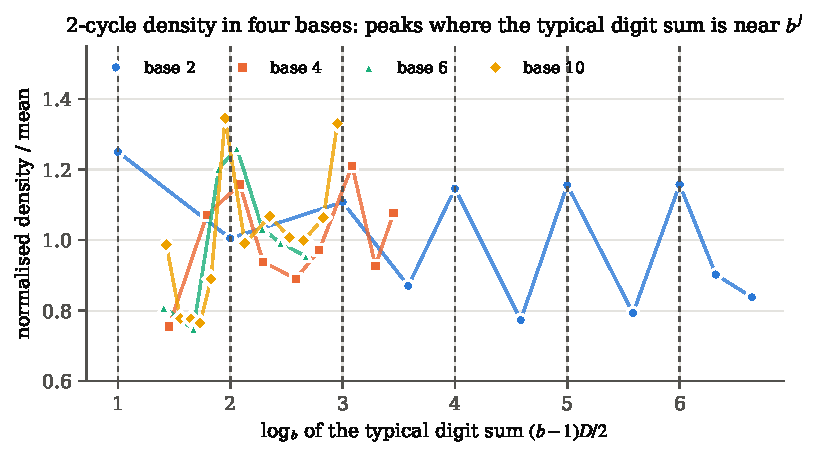
\includegraphics[width=0.92\textwidth]{figures/bases_resonance.pdf}
\caption{Exact normalised $2$-cycle densities $\sqrt{\ln D}\,T_b(D)/b^D$ (each
divided by its mean) in bases $2,4,6,10$, plotted against $\log_b$ of the
typical digit sum $(b-1)D/2$. In every base the peaks lie near integers, where
the typical digit sum is close to $b^j-1$ (Proposition~\ref{prop:resb}).}\label{fig:bases}
\end{figure}

Figure~\ref{fig:bases} shows exact counts in four bases. In base $2$ the
normalised density oscillates between about $0.09$ and $0.14$, with peaks at
$D=16,32,64,128$, where the typical digit sum $D/2$ is just below a power of
$2$, and troughs at $D=24,48,96$. Theorems~\ref{thm:oddbase}
and~\ref{thm:evenb} together give a complete picture at the level of
$2$-cycles: in odd bases the dynamics is trivial, and in every even base the
$2$-cycles have density of exact order $(\log D)^{-1/2}$, with resonances
located at the base-$b$ repunits $b^j-1$.

\section{Convergence}\label{sec:convergence}

We stress at the outset what is and is not proved. Every orbit computed so far
is eventually periodic, but we do \emph{not} prove that every orbit is
eventually periodic (Conjecture~\ref{conj:conv}). What we prove is an exact
reformulation: eventual periodicity is equivalent to boundedness of the digit
sums along the orbit (Theorem~\ref{thm:conv}).

\begin{lemma}[Crossing lemma]\label{lem:cross}
If a term $n<10^J$ of an orbit is followed by $f(n)\ge10^J$, then $n$ is odd
and $10^J-n\le s(n)$; if moreover $s(n)\le B<10^t$, the leading $J-t$ digits
of $n$ are nines, so $s(n)\ge9(J-t)$.
\end{lemma}

\begin{proof}
If $n$ were even, $f(n)=n-s(n)\le n<10^J$, a contradiction; so $n$ is odd and
$f(n)=n+s(n)\ge10^J$, i.e.\ $10^J-n\le s(n)$. If $s(n)\le B<10^t$ (with
$t<J$), then $10^J-10^t<10^J-B\le n<10^J$. Every integer in the interval
$(10^J-10^t,\,10^J)$ has exactly $J$ digits, of which the leading $J-t$ are
nines, since $10^J-10^t$ is the number formed by $J-t$ nines followed by $t$
zeros. Hence $s(n)\ge9(J-t)$.
\end{proof}

\begin{theorem}[Convergence criterion]\label{thm:conv}
The orbit of $n$ is eventually periodic if and only if the digit sums of its
terms are bounded. If they are bounded by $B<10^t$, every term is below
$10^J$ with $J=\max(\lceil\log_{10}(n+1)\rceil,\lfloor B/9\rfloor+t+1)$.
\end{theorem}

\begin{proof}
Eventually periodic orbits are finite. Conversely, $n<10^J$; if a term
reached $10^J$, its predecessor $m$ would satisfy
$s(m)\ge9(J-t)\ge9(\lfloor B/9\rfloor+1)>B$ by Lemma~\ref{lem:cross}. So the
orbit is bounded, hence eventually periodic.
\end{proof}

\begin{corollary}[Anatomy of a divergent orbit]
A divergent orbit contains, for infinitely many $J$, an odd term $10^J-x$
with $1\le x\le s(10^J-x)$: a block of nines followed by a short tail. Its
digit sums are unbounded.
\end{corollary}

\begin{proposition}[Ascents with small digit sum]\label{prop:uprun}
Let $9\mid n_0$, $n_0$ odd, $s(n_0)$ even and $s(n_0)<198$, and let
$n_0<n_1<\dots$ be the ascending run from $n_0$, i.e.\ the consecutive odd
terms $n_{j+1}=n_j+s(n_j)$. Then the run is finite. Along it the digit sum
never increases, except possibly at its last term, where it can exceed the
previous digit sum by $9$.
\end{proposition}

\begin{proof}
Every odd $n_j$ with $s(n_j)$ even is followed by the odd term
$n_{j+1}=n_j+s(n_j)$. If $s(n_j)$ is odd, then $n_j+s(n_j)$ is even, so $n_j$
is the last term of the run. Suppose $s(n_j)=S$ is even, a multiple of $9$, and
$18\le S\le180$, so $s(S)=9$. By Lemma~\ref{lem:carry},
$s(n_{j+1})=S+9-9C$ with $C=\C(n_j,S)\ge0$. If $C$ is odd, $s(n_{j+1})\le S$
is even and the run continues at a level that has not increased. If $C$ is
even, $s(n_{j+1})$ is odd, so $n_{j+1}$ is the last term. Its digit sum is
$S+9$ if $C=0$ and at most $S-9$ otherwise.\footnote{For example $8901\to8919$:
$s=18\to27$, after which $f(8919)=8946$ is even and $8919\leftrightarrow8946$
is a $2$-cycle.} By induction, every term before the last has an even digit
sum of at most $s(n_0)\le180$, and the last term has digit sum at most
$s(n_0)+9<198$. The run is increasing with bounded digit sums, so it is finite
by Lemma~\ref{lem:cross}, as in the proof of Theorem~\ref{thm:conv}.
\end{proof}

The next theorem removes the restriction to small levels for runs along
which the level does not change. It applies the carry-balance idea along an
arithmetic progression: while the level is constant, an ascent adds the same
number $9k$ at every step, and the digits above the lowest ones then behave
like a counter that must eventually pass a block of nines.

\begin{theorem}[Constant-level runs are short]\label{thm:shortruns}
Let $9\mid n_0$ have level $k\ge1$, let $\ell$ be the number of digits of $9k$
and $\kappa=\kappa(k)$. Suppose $n_0,n_1,\dots,n_r$ are consecutive terms of an
orbit that all have level $k$. Then
\[
  |n_r-n_0|<2\cdot10^{\ell+\kappa}\le2\cdot(90k)^2 .
\]
\end{theorem}

\begin{proof}
If $k$ is odd, each step adds or subtracts the odd number $9k$, so parity
alternates. An odd term $n_j$ goes up to $n_j+9k$, which is even, has level
$k$ and therefore returns to $n_j$; an even term likewise goes down and
returns. So the run alternates between two values, and
$|n_r-n_0|\le9k<2\cdot10^{\ell}$.

If $k$ is even, $9k$ is even and every term has the parity of $n_0$, so the
run is either ascending
($n_{j+1}=n_j+9k$, all $n_j$ odd) or descending ($n_{j+1}=n_j-9k$, all even);
consider an ascending run, the descending case being identical with borrows
and zeros in place of carries and nines. By Theorem~\ref{thm:level}, every step
produces exactly $\kappa$ carries. Write $n_j=q_j10^\ell+x_j$ with
$0\le x_j<10^\ell$. Since $9k<10^\ell$, each step increases $q$ by $0$ or $1$,
and by $1$ exactly when it carries out of column $\ell-1$; as $x$ grows by $9k$
on every step that does not increase $q$, $q$ increases at least once in every
$\lceil10^\ell/(9k)\rceil$ consecutive steps.

Suppose $q$ increases at least $10^\kappa$ times during the run. The values
$q_0,q_0+1,\dots,q_0+10^\kappa-1$ are then all taken, one of them, $q^*$, ends in
$\kappa$ nines, and the step that raises $q$ from $q^*$ to $q^*+1$ belongs to the
run. That step carries out of column $\ell-1$ and then through the $\kappa$
nines in columns $\ell,\dots,\ell+\kappa-1$, so it produces at least $\kappa+1$
carries, a contradiction. Hence $q$ increases at most $10^\kappa-1$ times, so
$r\le10^\kappa\lceil10^\ell/(9k)\rceil$ and
\[
  n_r-n_0=9k\,r\le9k\cdot10^\kappa\Bigl(\frac{10^\ell}{9k}+1\Bigr)
  =10^{\ell+\kappa}+9k\cdot10^\kappa<2\cdot10^{\ell+\kappa}.
\]
Finally $\kappa\le\ell$ (the digit sum of $9k$ is at most $9\ell$) and
$10^\ell\le90k$, so $10^{\ell+\kappa}\le(90k)^2$.
\end{proof}

The bound was checked on $228$ maximal constant-level runs in orbits of random
numbers with $30$ to $480$ digits: none came within $14\%$ of it. Since the
level of a $D$-digit number is at most $D$, every constant-level run moves the
orbit by $O(D^2)$, a negligible amount compared with $n$.

\paragraph{What is missing for global convergence.} Theorem~\ref{thm:shortruns}
does not by itself bound an \emph{ascent}, i.e.\ a maximal stretch on the odd
rail, because the level may change inside an ascent and stay even. For
$k\le10$ the only possible increase is to $k+1$, which leaves the rail, and
this gives Proposition~\ref{prop:uprun}. For larger $k$, $\kappa(k)\ge2$ allows
an increase by $2$ that keeps the rail, and such increases do occur: among
$448$ ascents in orbits of random numbers with $50$ to $800$ digits we
observed $14$ level increases by $2$ (and $244$ by $1$, at the end of an
ascent). The heights of these ascents nevertheless grew only linearly with
the number of digits (at most $39{,}240$ for $800$ digits). A proof of
Conjecture~\ref{conj:conv} along these lines would need to show that level
increases inside an ascent cannot accumulate, for example by controlling the
level along the counter $q$ above.

\subsection*{A computer-assisted proof for all starting values below explicit bounds}

Prefix lifting turns Conjecture~\ref{conj:conv}, restricted to a finite range,
into a finite check, provided the blocks are large enough that a single
constant-level run cannot cross one (Theorem~\ref{thm:shortruns}). We state it
for every even base $b$; recall that $f_b$ has the parity of the last digit.

\begin{theorem}[Block certificate]\label{thm:cert}
Let $b$ be even, $D>L\ge1$, $M=b^L$, $\sigma_{\max}=(b-1)(D-L)$ and
$E=\sigma_{\max}+(b-1)L+1$, and assume $\sigma_{\max}+(b-1)L<M$. For
$0\le\sigma\le\sigma_{\max}$ let $g_\sigma(x)=x\pm(\sigma+s_b(x))$ (plus for odd
$x$, minus for even $x$) on $[0,M)$. Suppose that for every such $\sigma$ no
$x<E$ is carried by iterating $g_\sigma$ to a value $\ge M$. Then every orbit of
$f_b$ starting at some $n<b^D$ stays below $(\lfloor n/M\rfloor+2)M$; in
particular it is bounded, hence eventually periodic, and
$\max(\text{orbit})-n<2M$.
\end{theorem}

\begin{proof}
Write each term as $H\cdot M+x$ with $0\le x<M$. Since $s_b(HM+x)=s_b(H)+s_b(x)$
and $HM+x\equiv x\pmod2$, as long as $H$ is unchanged the low part evolves by
$g_{s_b(H)}$; each step changes $x$ by less than $M$ (because
$s_b(HM+x)\le\sigma_{\max}+(b-1)L<M$ whenever $s_b(H)\le\sigma_{\max}$), so $H$
changes by at most $1$ per step, upwards exactly when $g_{s_b(H)}$ leaves
$[0,M)$ at the top. Right after such an upward step the new low part is
$x'=y+s_b(HM+y)-M<s_b(HM+y)\le\sigma_{\max}+(b-1)L<E$.

Let $H_0=\lfloor n/M\rfloor<b^{D-L}$. Suppose some term had high part
$H_0+2$, and consider the first such term. Its predecessor has high part
$H_0+1$, and the maximal stretch of the orbit at high part $H_0+1$ that
contains it began with an upward step from $H_0$ (it cannot have begun with
a downward step from $H_0+2$, which has not yet occurred, nor with $n$
itself). So that stretch starts at a low part $x'<E$ and leaves $[0,M)$ at the
top under $g_\sigma$ with $\sigma=s_b(H_0+1)$. As $H_0+1\le b^{D-L}$ we have
$\sigma\le\sigma_{\max}$, contradicting the hypothesis. Hence every term has
high part at most $H_0+1$, so the orbit is contained in $[0,(H_0+2)M)$. A
bounded orbit of a map on the integers is eventually periodic, and
$\max(\text{orbit})-n<(H_0+2)M-H_0M=2M$.
\end{proof}

The hypothesis is a finite computation: for each $\sigma$, the fate of every
$x\in[0,M)$ under $g_\sigma$ (absorbed at the top, absorbed at the bottom, or
periodic) is determined exactly by iterating the functional graph $2^r\ge M+2$
times with pointer doubling, in exact integer arithmetic.

\begin{theorem}[Eventual periodicity below explicit bounds]\label{thm:certres}
Every orbit of the binary map $f_2$ starting below $2^{3024}$, and every orbit
of the decimal map $f$ starting below $10^{2224}$, is eventually periodic. For
these starting values, $\max(\text{orbit})-n<2\cdot2^{24}$ and
$\max(\text{orbit})-n<2\cdot10^{8}$, respectively.
\end{theorem}

\begin{proof}
The hypothesis of Theorem~\ref{thm:cert} was verified by computer for the
parameters in Table~\ref{tab:cert}. The last row of each base uses the climb
method described below.
\end{proof}

\begin{table}[h]
\centering
\begin{tabular}{rrrrrr}
\toprule
base $b$ & all $n<$ & block $b^L$ & $\sigma_{\max}$ & entries checked $E$ & time\\
\midrule
$2$ & $2^{64}$ & $2^{16}$ & $48$ & $65$ & $1$\,s\\
$2$ & $2^{128}$ & $2^{18}$ & $110$ & $129$ & $3$\,s\\
$2$ & $2^{256}$ & $2^{20}$ & $236$ & $257$ & $28$\,s\\
$2$ & $2^{512}$ & $2^{22}$ & $490$ & $513$ & $4$\,min\\
$10$ & $10^{12}$ & $10^{5}$ & $63$ & $109$ & $1$\,s\\
$10$ & $10^{20}$ & $10^{6}$ & $126$ & $181$ & $14$\,s\\
$10$ & $10^{30}$ & $10^{7}$ & $207$ & $271$ & $3.5$\,min\\
\midrule
$2$ & $2^{3024}$ & $2^{24}$ & $3000$ & $3025$ & $30$\,s$^*$\\
$10$ & $10^{2224}$ & $10^{8}$ & $19944$ & $20017$ & $2$\,min$^{*\dagger}$\\
\bottomrule
\end{tabular}
\caption{Parameters for which the block certificate (Theorem~\ref{thm:cert})
was verified, with running times on a laptop. Rows marked $^*$ use the
climb method: every orbit is followed on the half-line and its maximum is
compared with $b^L$. $^\dagger$On $8$ cores.}\label{tab:cert}
\end{table}

\emph{Climb method.} The hypothesis of Theorem~\ref{thm:cert} only concerns
the finite low maps, and $g_\sigma$ on $[0,b^L)$ agrees with the half-line map
$x\mapsto x\pm(\sigma+s_b(x))$ until the orbit leaves the block. It therefore
suffices to follow each entry $x_0<E$ on the half-line, until it falls below
$0$ or closes a cycle, and to check that its maximum is below $b^L$. Memoising
the maximum over each orbit makes this cost roughly linear in the number of
states actually visited, rather than $b^L$. This removes the memory
bottleneck of the block arrays. In base $10$ with $L=8$, for every
$\sigma\le19{,}944$ and every entry below $E=20{,}017$, the highest point reached
is $20{,}020{,}006$ (at $\sigma=19{,}943$), below $10^8$. In base $2$ with $L=24$,
for $\sigma\le3000$, it is $2{,}107{,}392<2^{24}$. These give the last two rows of
Table~\ref{tab:cert}. Figure~\ref{fig:climb} shows the maximum climb as a
function of $\sigma$. It is not smooth: a slowly rising baseline carries sharp
spikes when $\sigma$ is just below a multiple of $1000$, about $2\cdot10^6$ at
even thousands, $10^7$ near $10^4$ and $2\cdot10^7$ near $2\cdot10^4$. There the
step $\sigma+s(x)$ is just below a round number, and carries propagate
through long blocks of nines: this is the resonance of
Section~\ref{sec:resonance}, now acting on climbs. The next spike makes $L=8$
insufficient. At $\sigma=19{,}961$ an orbit reaches about $2\cdot10^8$, so
extending the range needs $L=9$. The reported range is therefore the largest
this block size certifies, not an artefact of stopping early.

\paragraph{Verification protocol.} The \emph{proof} consists of exactly two
finite computations, the last two rows of Table~\ref{tab:cert}. Their inputs
are $(b,\sigma_{\max},L)=(10,19944,8)$ and $(2,3000,24)$, and their outputs are
the highest points $20{,}020{,}006<10^8$ and $2{,}107{,}392<2^{24}$. Every other
computation in this section is a \emph{cross-check}. These are the block
method on small parameters, direct orbit enumeration, and the deliberately
failing case $(2,16,8)$, which make implementation errors unlikely but prove
nothing. The two proof computations are recomputed by a standalone checker,
\texttt{verify\_certificates.py}, under $100$ lines that share no code with the
rest of the package. It follows each entry $x_0<E$ until the orbit becomes
negative or reaches a state already seen. Because the highest point of a
forward orbit depends only on its starting state, storing it for every state
visited (memoisation) is exact. If the program finishes, every orbit has been
followed completely. It reproduces all $19{,}945$ per-$\sigma$ maxima of
Figure~\ref{fig:climb} exactly, and reports failure on $(2,16,8)$. The archived
release lists SHA-256 hashes of the checker, the certificate outputs and the
manuscript source.

\begin{figure}[t]
\centering
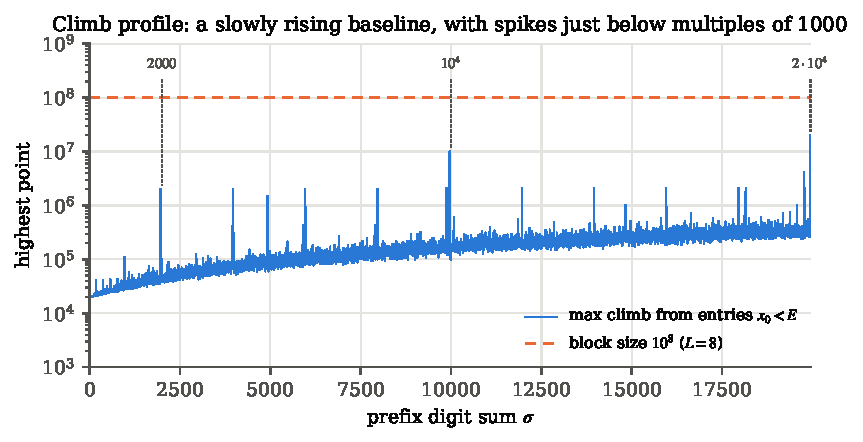
\includegraphics[width=0.9\textwidth]{figures/climb_profile.pdf}
\caption{Maximum climb of the low maps $g_\sigma$ from all entries
$x_0<E=20{,}017$, against $\sigma$ (base $10$, $L=8$). Every value lies below
the block size $10^8$, which proves Theorem~\ref{thm:certres} for all
$n<10^{2224}$. Spikes occur just below multiples of $1000$, where the step is
close to a round number.}\label{fig:climb}
\end{figure} On the six small parameter sets used below, the climb
method and the block method give identical verdicts, including the failure at
$(2,16,8)$.

These ranges exceed exhaustive enumeration ($n\le2\cdot10^6$) by a factor of
about $10^{2218}$ in base $10$. Two checks guard against errors in the
implementation. First, for small parameters
($(b,D,L)=(2,18,9),(4,8,5),(10,5,3),(10,6,4)$) every orbit starting below
$b^D$ was followed directly, and its high part never exceeded $H_0+1$, as the
theorem asserts. Second, the certificate is not vacuous: for $(b,D,L)=(2,16,8)$
it fails, and direct computation shows that some orbit below $2^{16}$ does
climb two blocks.

The block size needed grows only logarithmically: $L=2\log_2D+4$ in base $2$
for $D=64,128,256,512$, and $L=5,6,7$ for $D=12,20,30$ in base $10$. The
following lemma explains why a check at one scale controls larger scales.
Write $\mathrm{Bad}_L(\sigma;W)$ if some $x<W$ reaches the top exit of
$[0,b^L)$ under $g_\sigma$.

\begin{lemma}[Scale reduction]\label{lem:scale}
Let $L>L'\ge1$, $b$ even, and $\sigma+(b-1)L\le W\le b^{L'}$. If
$\mathrm{Bad}_L(\sigma;W)$, then $\mathrm{Bad}_{L'}(\sigma+j;W)$ for every
$j\in\{0,1,\dots,(b-1)(L-L')\}$.
\end{lemma}

\begin{proof}
Write $x=h\,b^{L'}+y$ with $0\le y<b^{L'}$. Then
$s_b(x)=s_b(h)+s_b(y)$ and $x\equiv y\pmod 2$, so while $h$ is fixed the orbit
of $g_\sigma$ follows $g_{\sigma+s_b(h)}$ on $[0,b^{L'})$. Every step is at
most $\sigma+(b-1)L<b^{L'}$, so $h$ changes by $\pm1$ at a time. An orbit
starting at $x<W\le b^{L'}$ (so $h=0$) and leaving $[0,b^L)$ at the top must
cross from $h$ to $h+1$ for every $h<b^{L-L'}$. Fix such an $h$ and consider
the last entry into sub-block $h$ before the first crossing to $h+1$. For
$h=0$ it is the start $y=x<W$. For $h\ge1$ it comes from $h-1$, since $h+1$
has not been visited, and the entry point satisfies
$y<\text{step}\le\sigma+(b-1)L\le W$. From $y$ the map
$g_{\sigma+s_b(h)}$ carries the orbit to the top of the sub-block, so
$\mathrm{Bad}_{L'}(\sigma+s_b(h);W)$. As $h$ ranges over
$[0,b^{L-L'})$, $s_b(h)$ takes every value in $\{0,\dots,(b-1)(L-L')\}$.
\end{proof}

So the bad set at scale $L$ is contained in the set of $\sigma$ whose whole
window $[\sigma,\sigma+(b-1)(L-L')]$ is bad at scale $L'$. A single good
parameter at a small scale therefore certifies $(b-1)(L-L')+1$ parameters at
every larger scale. Numerically, though, the bad set at a fixed scale is not
sparse. Once $\sigma$ exceeds roughly $b^{L/2}$, almost every $\sigma$ is bad,
so the lemma speeds up the computation but does not by itself give a proof.

The quantity that governs the problem is $L_{\min}(\sigma)$, the least $L$
with no $x<\sigma+(b-1)L+1$ exiting at the top. Every $\sigma\le\theta_L$
satisfies $L_{\min}(\sigma)\le L$, where
\[
\begin{array}{c|cccc|ccccc}
b & 10&10&10&10 & 2&2&2&2&2\\
L & 3&4&5&6 & 10&12&14&16&18\\
\theta_L & 69&179&963&1952 & 54&113&244&495&1010\\
b^L/\theta_L^2 & 0.21&0.31&0.11&0.26 & 0.35&0.32&0.28&0.27&0.26
\end{array}
\]
In both bases the block needed is quadratic in $\sigma$, with
$b^{L_{\min}}\approx\sigma^2/4$. This is the order of the height
$2b^{\ell+\kappa}\le2((b-1)bk)^2$ of a constant-level run in
Theorem~\ref{thm:shortruns}. It suggests that climbs from the bottom are no
higher than single constant-level runs, so the level changes inside an ascent
do not compound. Conjecture~\ref{conj:conv} would follow from the uniform
quantitative strengthening below.

For the statement we use the half-line map
$\bar g_\sigma(x)=x+\sigma+s_b(x)$ ($x$ odd), $x-\sigma-s_b(x)$ ($x$ even), on
$\mathbb Z_{\ge0}$, with orbits stopped when they become negative. It does not
involve a block length; $g_\sigma$ on $[0,b^L)$ agrees with it until the
orbit leaves the block.

\begin{conjecture}[Quadratic climbs]\label{conj:quad}
There is an absolute constant $c$ such that for every even $b$, every
$\sigma\ge0$ and every $X\ge0$, every orbit of $\bar g_\sigma$ that starts at
some $x_0\le X$ stays below $c\,(\sigma+X+1)^2$.
\end{conjecture}

Conjecture~\ref{conj:quad} is a strengthening of Conjecture~\ref{conj:conv},
not a reduction of it. Since $\bar g_0=f$, the case $\sigma=0$ already says
that every orbit of $f$ starting at $x_0\le X$ stays below $c(X+1)^2$, a
quantitative form of Conjecture~\ref{conj:conv}. What the conjecture adds is
uniformity in $\sigma$, which is the form the block certificate needs. That
it implies Conjecture~\ref{conj:conv} can be seen directly, or through
Theorem~\ref{thm:cert}, as follows. Given $D$,
choose $L$ minimal with $b^L>c\,(2(b-1)D+1)^2$, so $L=O(\log D)$, and apply
Theorem~\ref{thm:cert}. Its hypothesis concerns $\sigma\le\sigma_{\max}=(b-1)(D-L)$
and entries $x_0<E=\sigma_{\max}+(b-1)L+1$. With $X=E$ the conjecture bounds
every such orbit by $c(\sigma_{\max}+E+1)^2\le c(2(b-1)D+1)^2<b^L$, so no orbit
reaches the top of the block. The data of Theorem~\ref{thm:certres} are
consistent with $c=1$: for $\sigma\le19{,}944$ and $X=E$ the highest point is
$20{,}020{,}006<(19{,}944+20{,}017)^2$ in base $10$, and for $\sigma\le3000$ it is
$2{,}107{,}392<(3000+3025)^2$ in base $2$. For
$10\le\sigma\le3000$ and all entries $x\le\sigma+(b-1)\cdot8$ (base $10$) or
$x\le\sigma+24$ (base $2$), about $4.7$ million starting points in each base,
the highest point is below $1.71(\sigma+1)^2$ in base $10$ and
$1.19(\sigma+1)^2$ in base $2$. The number of separate up-runs in a climb is
not bounded, however. It reaches $19$ in base $10$ and $61$ in base $2$, with
up to $33$ and $61$ level changes. So a proof cannot simply count runs: it must
show that successive runs do not stack. The conjecture concerns only the
maps $\bar g_\sigma$, with no dynamics of the prefix. Theorem~\ref{thm:shortruns} proves it
for runs at constant level. What remains is to control level increases inside
an ascent, which we do not know how to do.

The structure above explains convergence heuristically: regular steps are
translations that Theorem~\ref{thm:reverse} pairs into ascents and mirrored
descents, so net drift can only come from exceptional carries, which require
long blocks of nines. Numerically, every orbit from $n\le2\cdot10^6$ is
eventually periodic, the largest excursion $\max(\mathrm{orbit})-n$ there is
$777$ (at $n=998457$), and for $300$ random starts (Python
\texttt{random.Random(0)}) with each of
$10,\dots,400$ digits the excursion grows roughly linearly in the number of
digits (Figure~\ref{fig:excursion}).

\begin{figure}[t]
\centering
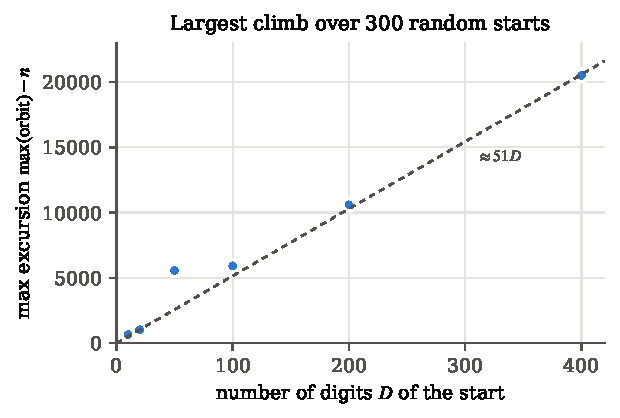
\includegraphics[width=0.55\textwidth]{figures/excursion.pdf}
\caption{Largest excursion over $300$ random starting values for each number
of digits.}\label{fig:excursion}
\end{figure}

\begin{conjecture}\label{conj:conv}
Every orbit of $f$ is eventually periodic; equivalently, digit sums are
bounded along every orbit.
\end{conjecture}

\begin{remark}
Theorem~\ref{thm:lift} suggests a computer-assisted proof for $n<10^D$: track
the low map $g_\sigma$ and show that the prefix cannot climb indefinitely. A
coarse version (after the prefix increases it cannot increase again before
decreasing) fails for sparse clusters of $\sigma$; a finer version tracking the
last digits of $H$ and the side from which each level is entered remains to
be carried out.
\end{remark}

\section{Cycle statistics}

Two different quantities are easy to confuse here: the number of
\emph{distinct cycles} of a given length, and the proportion of
\emph{starting values} whose orbit enters a cycle of that length. They can
differ substantially, because basins have very different sizes.
Table~\ref{tab:cycles} and Figure~\ref{fig:basins} give both.

Table~\ref{tab:corrected} counts the distinct cycles reached from multiples
of $9$ up to $N$ (each cycle counted once, regardless of the point at which it
is entered) and the number of steps before the orbit enters its cycle.

\begin{table}[h]
\centering
\begin{tabular}{rrrrr}
\toprule
$N$ & distinct cycles & mean steps & std.\ steps & max steps\\
\midrule
500 & 20 & 0.47 & 0.78 & 3\\
1{,}000 & 26 & 1.95 & 2.97 & 13\\
10{,}000 & 171 & 1.35 & 1.70 & 13\\
100{,}000 & 2{,}037 & 1.16 & 1.44 & 13\\
200{,}000 & 4{,}149 & 1.16 & 1.51 & 27\\
\bottomrule
\end{tabular}
\caption{Orbits of the multiples of $9$ up to $N$: number of distinct cycles
reached, and statistics of the number of steps before entering the cycle
(exact enumeration).}\label{tab:corrected}
\end{table}

\begin{table}[t]
\centering
\small
\begin{tabular}{rrrrl}
\toprule
length & \#cycles & \% of cycles & \% of starts & smallest example\\
\midrule
2 & 37374 & 86.5 & 72.3 & $9,\ 18$\\
3 & 81 & 0.19 & 0.70 & $8991,\ 9018,\ 9000$\\
4 & 4759 & 11.0 & 20.7 & $2871,\ 2889,\ 2916,\ 2898$\\
5 & 72 & 0.17 & 0.57 & $289953,\ 289989,\ 290034,\ 290016,\ 289998$\\
8 & 605 & 1.40 & 2.64 & $89793,\ 89829,\ \dots,\ 89820$\\
14 & 17 & 0.04 & 0.20 & $89991,\ 90027,\ \dots,\ 90000$\\
15 & 284 & 0.66 & 2.79 & $1791,\ 1809,\ \dots,\ 1899,\ 1926,\ \dots,\ 1800$\\
16 & 18 & 0.04 & 0.16 & $189783,\ 189819,\ \dots,\ 189810$\\
\bottomrule
\end{tabular}
\caption{Cycles other than the fixed point $\{0\}$ reached from
$1\le n\le2\cdot10^6$: number of distinct cycles, their share of all
$43{,}210$ cycles, the share of starting values $n$ whose orbit enters a
cycle of that length (only the six starts $1,2,3,4,6,8$ reach $\{0\}$), and the cycle of
smallest minimum for each length.}\label{tab:cycles}
\end{table}

\begin{figure}[t]
\centering
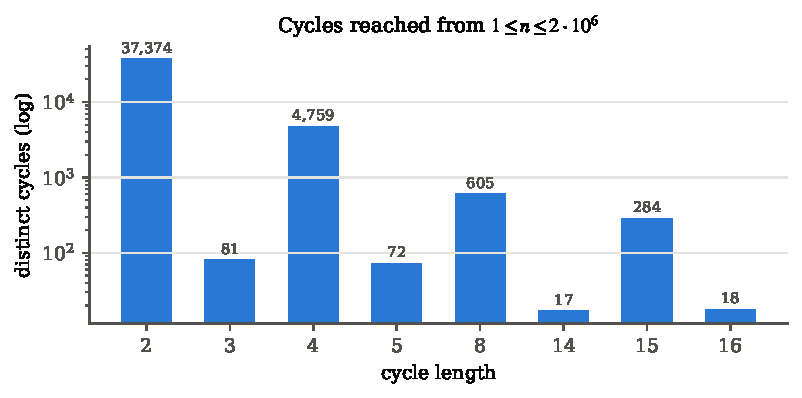
\includegraphics[width=0.75\textwidth]{figures/cycle_lengths.pdf}
\caption{Distribution of cycle lengths (logarithmic scale).}\label{fig:lengths}
\end{figure}

\begin{figure}[!htbp]
\centering
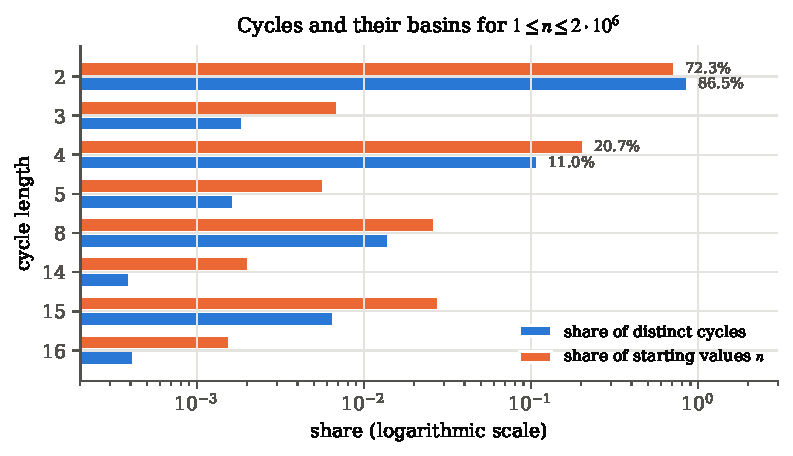
\includegraphics[width=0.8\textwidth]{figures/basins.pdf}
\caption{Share of distinct cycles (blue) and of starting values (orange) by
cycle length, for $1\le n\le2\cdot10^6$. The $2$-cycles are $86.5\%$ of the
cycles but attract only $72.3\%$ of the starts; $4$-, $8$- and $15$-cycles have
larger basins than their numbers suggest.}\label{fig:basins}
\end{figure}

Table~\ref{tab:cycles} and Figure~\ref{fig:lengths} list the cycles found.
The statement in the introduction that $2$-cycles dominate refers to the
number of distinct cycles; by basin size they account for about
seven-tenths of all starting values.
Odd lengths occur; which lengths are possible, and how the turns produce
them, is not yet classified. In the $15$-cycle the ascent
adds $18$ six times and $27$ once and the descent subtracts $18$ seven times
and $9$ once, both totalling $135$.

\clearpage
\section{Open problems}
\begin{enumerate}
\item Prove Conjecture~\ref{conj:conv}. It is proved below $10^{2224}$
  (Theorem~\ref{thm:certres}); by Theorem~\ref{thm:cert} the general case would
  follow from the absence of upward crossings for the finite maps $g_\sigma$
  with blocks of size $b^{O(\log\sigma)}$. By Theorem~\ref{thm:shortruns} it
  would also suffice to show that level increases inside an ascent cannot
  accumulate. The same question can be asked in every even base; base $2$,
  where the digit sum is the number of ones, may be the most tractable case.
\item Corollary~\ref{cor:osc} determines the limit points of the
  normalised $2$-cycle density. Extend the oscillation law to every even base;
  the analogue of Lemma~\ref{lem:exactvar} holds with $10$ replaced by $b$,
  and the extremal problem of Lemma~\ref{lem:kappa} changes with $b$.
\item Do \emph{all} cycles, not only $2$-cycles, have density zero? In the
  census, $2$-cycles are about $86\%$ of all \emph{distinct} cycles, but
  points on longer cycles are not rare. Exhaustively, $5.0\%$, $5.2\%$ and
  $5.2\%$ of $n\le N$ are periodic for $N=10^5,10^6,10^7$, and the share of
  them on $2$-cycles falls from $73\%$ to $60\%$. Sampling $40{,}000$ random
  $D$-digit numbers gives periodic proportions of $5.7\%$, $4.5\%$, $4.9\%$,
  $4.4\%$, $5.0\%$, $4.3\%$ and $4.2\%$ (standard error $0.1\%$) for
  $D=8,16,\dots,512$, with $4$-cycles about as frequent as $2$-cycles and
  apparently oscillating with $D$. The data therefore neither confirm nor
  refute density zero. The natural conjecture is that the periodic proportion
  is of order $(\log D)^{-1/2}$, like that of $2$-cycles, which would make the
  decay invisible at these sizes. For a $4$-cycle $a\to b\to c\to d\to a$ with two ascending and two
  descending steps, closure means $s(a)+s(b)=s(c)+s(d)$; by
  Lemma~\ref{lem:carry} this is a linear condition on three carry and borrow
  counts, $\C(a,s(a))$, $\C(b,s(b))$ and $\B(c,s(c))$, which depend on
  overlapping low digits. The switch argument of Lemma~\ref{lem:switch}
  handles one such count; a proof for $4$-cycles needs a \emph{joint}
  anti-concentration bound for these coupled counts.
\item Determine the profile $c_L(\sigma)$ analytically, and classify the
  possible cycle lengths.
\item Explain the rare cycles with two ascending runs.
\end{enumerate}

\section*{Data and code}
All computations are reproducible with the accompanying Python package
(\texttt{digitdyn}), available at
\url{https://github.com/rudraneel93/Digital-Root} (directory
\texttt{digitdyn}) and archived on Zenodo as release v1.0.1,
\href{https://doi.org/10.5281/zenodo.23938785}{doi:10.5281/zenodo.23938785}~\cite{digitdynZenodo}. It
contains: the exhaustive orbit and cycle census
(Proposition~\ref{prop:census}, Tables~\ref{tab:cycles}
and~\ref{tab:corrected}); the digit dynamic programme for $T(D)$
(Table~\ref{tab:density}), tested against exhaustive enumeration for
$D\le5$; the prefix-lifting counter (Theorem~\ref{thm:lift},
Corollary~\ref{cor:lifterr}); the carry-resonance computation
(Theorem~\ref{thm:resrig}); exact checks of
Theorems~\ref{thm:self}, \ref{thm:level}, \ref{thm:reverse}
and~\ref{thm:balance}; the block and climb certificates of
Theorem~\ref{thm:certres}, with their outputs; the exact carry-variance and
oscillation-law computations (Section~\ref{sec:osclaw}); the basin census
(Table~\ref{tab:cycles}); a test suite of $59$ tests; a single script that
regenerates every table and figure; and SHA-256 hashes of the released
sources and certificate outputs. All computations were run on an Apple M1
laptop with 8\,GB of memory, using Python~3.11.9, NumPy~1.26.4 and
Matplotlib~3.10.6. The certificate for $2^{3024}$ takes under a minute, and the one for
$10^{2224}$ about two minutes on $8$ cores; the slowest step of the full reproduction is the
oscillation table (Table~\ref{tab:osc}), which evaluates the main term up to
$D\approx6\cdot10^7$. Throughout the paper we distinguish \emph{theorems}
(proved), \emph{computational statements} (exact computations over a stated
finite range) and \emph{conjectures}.

\begin{thebibliography}{99}
\bibitem{DiaconisFreedman} P.~Diaconis and D.~Freedman, Finite exchangeable
  sequences, \emph{Ann. Probab.} \textbf{8} (1980), 745--764.
\bibitem{MitzenmacherUpfal} M.~Mitzenmacher and E.~Upfal, \emph{Probability and
  Computing: Randomized Algorithms and Probabilistic Analysis}, Cambridge
  University Press, 2005.
\bibitem{Hoeffding} W.~Hoeffding, Probability inequalities for sums of bounded
  random variables, \emph{J. Amer. Statist. Assoc.} \textbf{58} (1963), 13--30.
\bibitem{BassilyKatai} N.~L.~Bassily and I.~K\'atai, Distribution of the values
of $q$-additive functions on polynomial sequences, \emph{Acta Math.\ Hungar.}
\textbf{68} (1995), 353--361.
\bibitem{DolgopyatSarig} D.~Dolgopyat and O.~M.~Sarig, \emph{Local Limit Theorems
for Inhomogeneous Markov Chains}, Lecture Notes in Mathematics \textbf{2331},
Springer, 2023.
\bibitem{DrmotaGajdosik} M.~Drmota and J.~Gajdosik, The distribution of the
sum-of-digits function, \emph{J.\ Th\'eor.\ Nombres Bordeaux} \textbf{10} (1998),
17--32.
\bibitem{MauduitRivat} C.~Mauduit and J.~Rivat, Sur un probl\`eme de Gelfond:
la somme des chiffres des nombres premiers, \emph{Ann.\ of Math.} \textbf{171}
(2010), 1591--1646.
\bibitem{Dobrushin} R.~L.~Dobrushin, Central limit theorem for nonstationary
Markov chains~I,~II, \emph{Theory Probab.\ Appl.} \textbf{1} (1956), 65--80 and
329--383.
\bibitem{SethuramanVaradhan} S.~Sethuraman and S.~R.~S.~Varadhan, A martingale
proof of Dobrushin's theorem for non-homogeneous Markov chains,
\emph{Electron.\ J.\ Probab.} \textbf{10} (2005), 1221--1235.
\bibitem{Hoggar} S.~G.~Hoggar, Chromatic polynomials and logarithmic
  concavity, \emph{J. Combin. Theory Ser. B} \textbf{16} (1974), 248--254.
\bibitem{Petrov} V.~V.~Petrov, \emph{Sums of Independent Random Variables},
  Springer, 1975.
\bibitem{Rogozin} B.~A.~Rogozin, On the increase of dispersion of sums of
  independent random variables, \emph{Theory Probab. Appl.} \textbf{6} (1961),
  97--99.
\bibitem{BorodinDiaconisFulman} A.~Borodin, P.~Diaconis and J.~Fulman, On adding a
  list of numbers (and other one-dependent determinantal processes),
  \emph{Bull. Amer. Math. Soc.} \textbf{47} (2010), 639--670.
\bibitem{DiaconisShaoSoundararajan} P.~Diaconis, X.~Shao and K.~Soundararajan,
  Carries, group theory, and additive combinatorics, \emph{Amer. Math.
  Monthly} \textbf{121} (2014), 674--688.
\bibitem{DiaconisFulman} P.~Diaconis and J.~Fulman, Carries, shuffling, and
  symmetric functions, \emph{Adv. in Appl. Math.} \textbf{43} (2009), 176--196.
\bibitem{Holte} J.~M.~Holte, Carries, combinatorics, and an amazing matrix,
  \emph{Amer. Math. Monthly} \textbf{104} (1997), 138--149.
\bibitem{Kaprekar} D.~R.~Kaprekar, \emph{The Mathematics of New Self-Numbers},
  Devlali, 1963.
\bibitem{Kummer} E.~E.~Kummer, \"Uber die Erg\"anzungss\"atze zu den
  allgemeinen Reciprocit\"atsgesetzen, \emph{J. Reine Angew. Math.}
  \textbf{44} (1852), 93--146.
\bibitem{Lagarias} J.~C.~Lagarias, The $3x+1$ problem and its
  generalizations, \emph{Amer. Math. Monthly} \textbf{92} (1985), 3--23.
\bibitem{OEIS-A003052} OEIS Foundation, Sequence A003052 (self numbers),
  \url{https://oeis.org/A003052}.
\bibitem{digitdynZenodo} R.~Das, \texttt{digitdyn}: code and data for
  ``Carries, Rails and Resonance'', version v1.0.1, Zenodo (2026),
  \url{https://doi.org/10.5281/zenodo.23938785}.
\bibitem{OEIS-A124176} E.~Angelini, Sequence A124176, The On-Line Encyclopedia
  of Integer Sequences (2006), \url{https://oeis.org/A124176}.
\bibitem{OEIS-A124177} E.~Angelini, Sequence A124177, The On-Line Encyclopedia
  of Integer Sequences (2006), \url{https://oeis.org/A124177}.
\bibitem{OEIS-A243260} OEIS Foundation, Sequence A243260,
  \url{https://oeis.org/A243260}.
\bibitem{OEIS-A004207} OEIS Foundation, Sequence A004207,
  \url{https://oeis.org/A004207}.
\end{thebibliography}

\end{document}
